\chapter{Investigation of illicit drugs in PTR-MS: Other drugs}\label{chapter:drugs}
\markboth{Investigation of illicit drugs in PTR-MS: Other drugs}{}

This chapter comprises a set of PTR-MS results that, whilst still of interest, could not be included in the main chapters of this thesis.


\section{Reduced electric field study}
The chemical composition, molecular weight and structure of 
3,4-methylenedioxymethamphetamine (MDMA),
morphine, 
codeine, 
heroin, 
cannabinol (CBN), 
delta-9-tetrahydrocannabinol ($\Delta$-9-THC)
and 
cannabidiol (CBD)
are given in \autoref{tab:DRs_structs}.
%
The product ion distributions as a function of the reduced electric field and the drift voltage for these substances are given in  figures \ref{fig:DR_mdma} to \ref{fig:DR_CBD}.

%\textbf{150$^\circ$, pressure 1 mbar?, TDU....}





\begin{table}
\centering
\caption{Chemical composition, molecular weight and structure of MDMA, morphine, codeine, heroin, CBN, $\Delta$-9-THC and CBD.}
\begin{tabular}{lccc}
\textbf{Compound} & \textbf{Formula} &\textbf{MW (g/mol)} &  \textbf{Structure} \\ 
\toprule
MDMA & C$_{11}$H$_{15}$NO$_2$ & 193 &  
\begin{minipage}[c]{0.3\linewidth}\centering
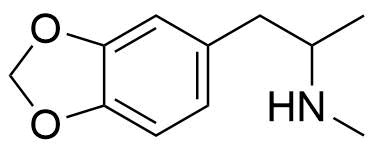
\includegraphics[height=0.05\textheight]{pics/other_drugs/MDMA_struct.png}\end{minipage}\\ \midrule
Morphine & C$_{17}$H$_{19}$NO$_3$ & 285 &  
\begin{minipage}[c]{0.3\linewidth}\centering
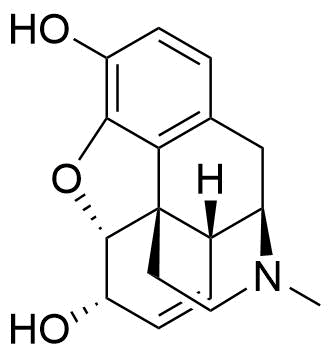
\includegraphics[height=0.12\textheight]{pics/other_drugs/morphine_struct.png}\end{minipage}\\ \midrule
Codeine & C$_{18}$H$_{21}$NO$_3$ & 299 &  
\begin{minipage}[c]{0.3\linewidth}\centering
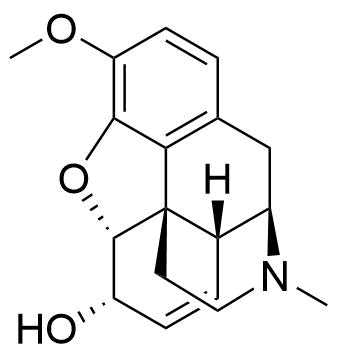
\includegraphics[height=0.12\textheight]{pics/other_drugs/codeine_struct.png}\end{minipage}\\ \midrule
Heroin & C$_{21}$H$_{23}$NO$_5$ & 369 &  
\begin{minipage}[c]{0.3\linewidth}\centering
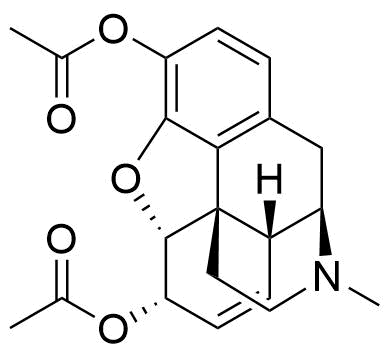
\includegraphics[height=0.12\textheight]{pics/other_drugs/heroin_struct.png}\end{minipage}\\ \midrule
CBN & C$_{21}$H$_{26}$O$_2$ & 310 &  
\begin{minipage}[c]{0.3\linewidth}\centering
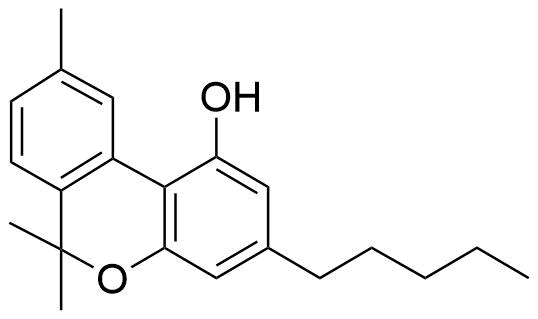
\includegraphics[height=0.1\textheight]{pics/other_drugs/CBN_struct.png}\end{minipage}\\ \midrule
$\Delta$-9-THC & C$_{21}$H$_{30}$O$_2$ & 314 &  
\begin{minipage}[c]{0.3\linewidth}\centering
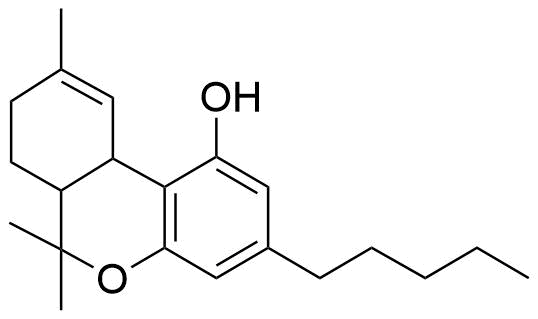
\includegraphics[height=0.1\textheight]{pics/other_drugs/THC_struct.png}\end{minipage}\\ \midrule
CBD & C$_{21}$H$_{30}$O$_2$ & 314 &  
\begin{minipage}[c]{0.3\linewidth}\centering
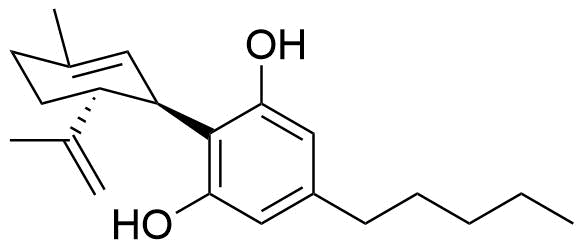
\includegraphics[height=0.1\textheight]{pics/other_drugs/CBD_struct.png}\end{minipage}\\ 
\bottomrule
\end{tabular}
\label{tab:DRs_structs}
\end{table}



\begin{figure}[htb]
\centering
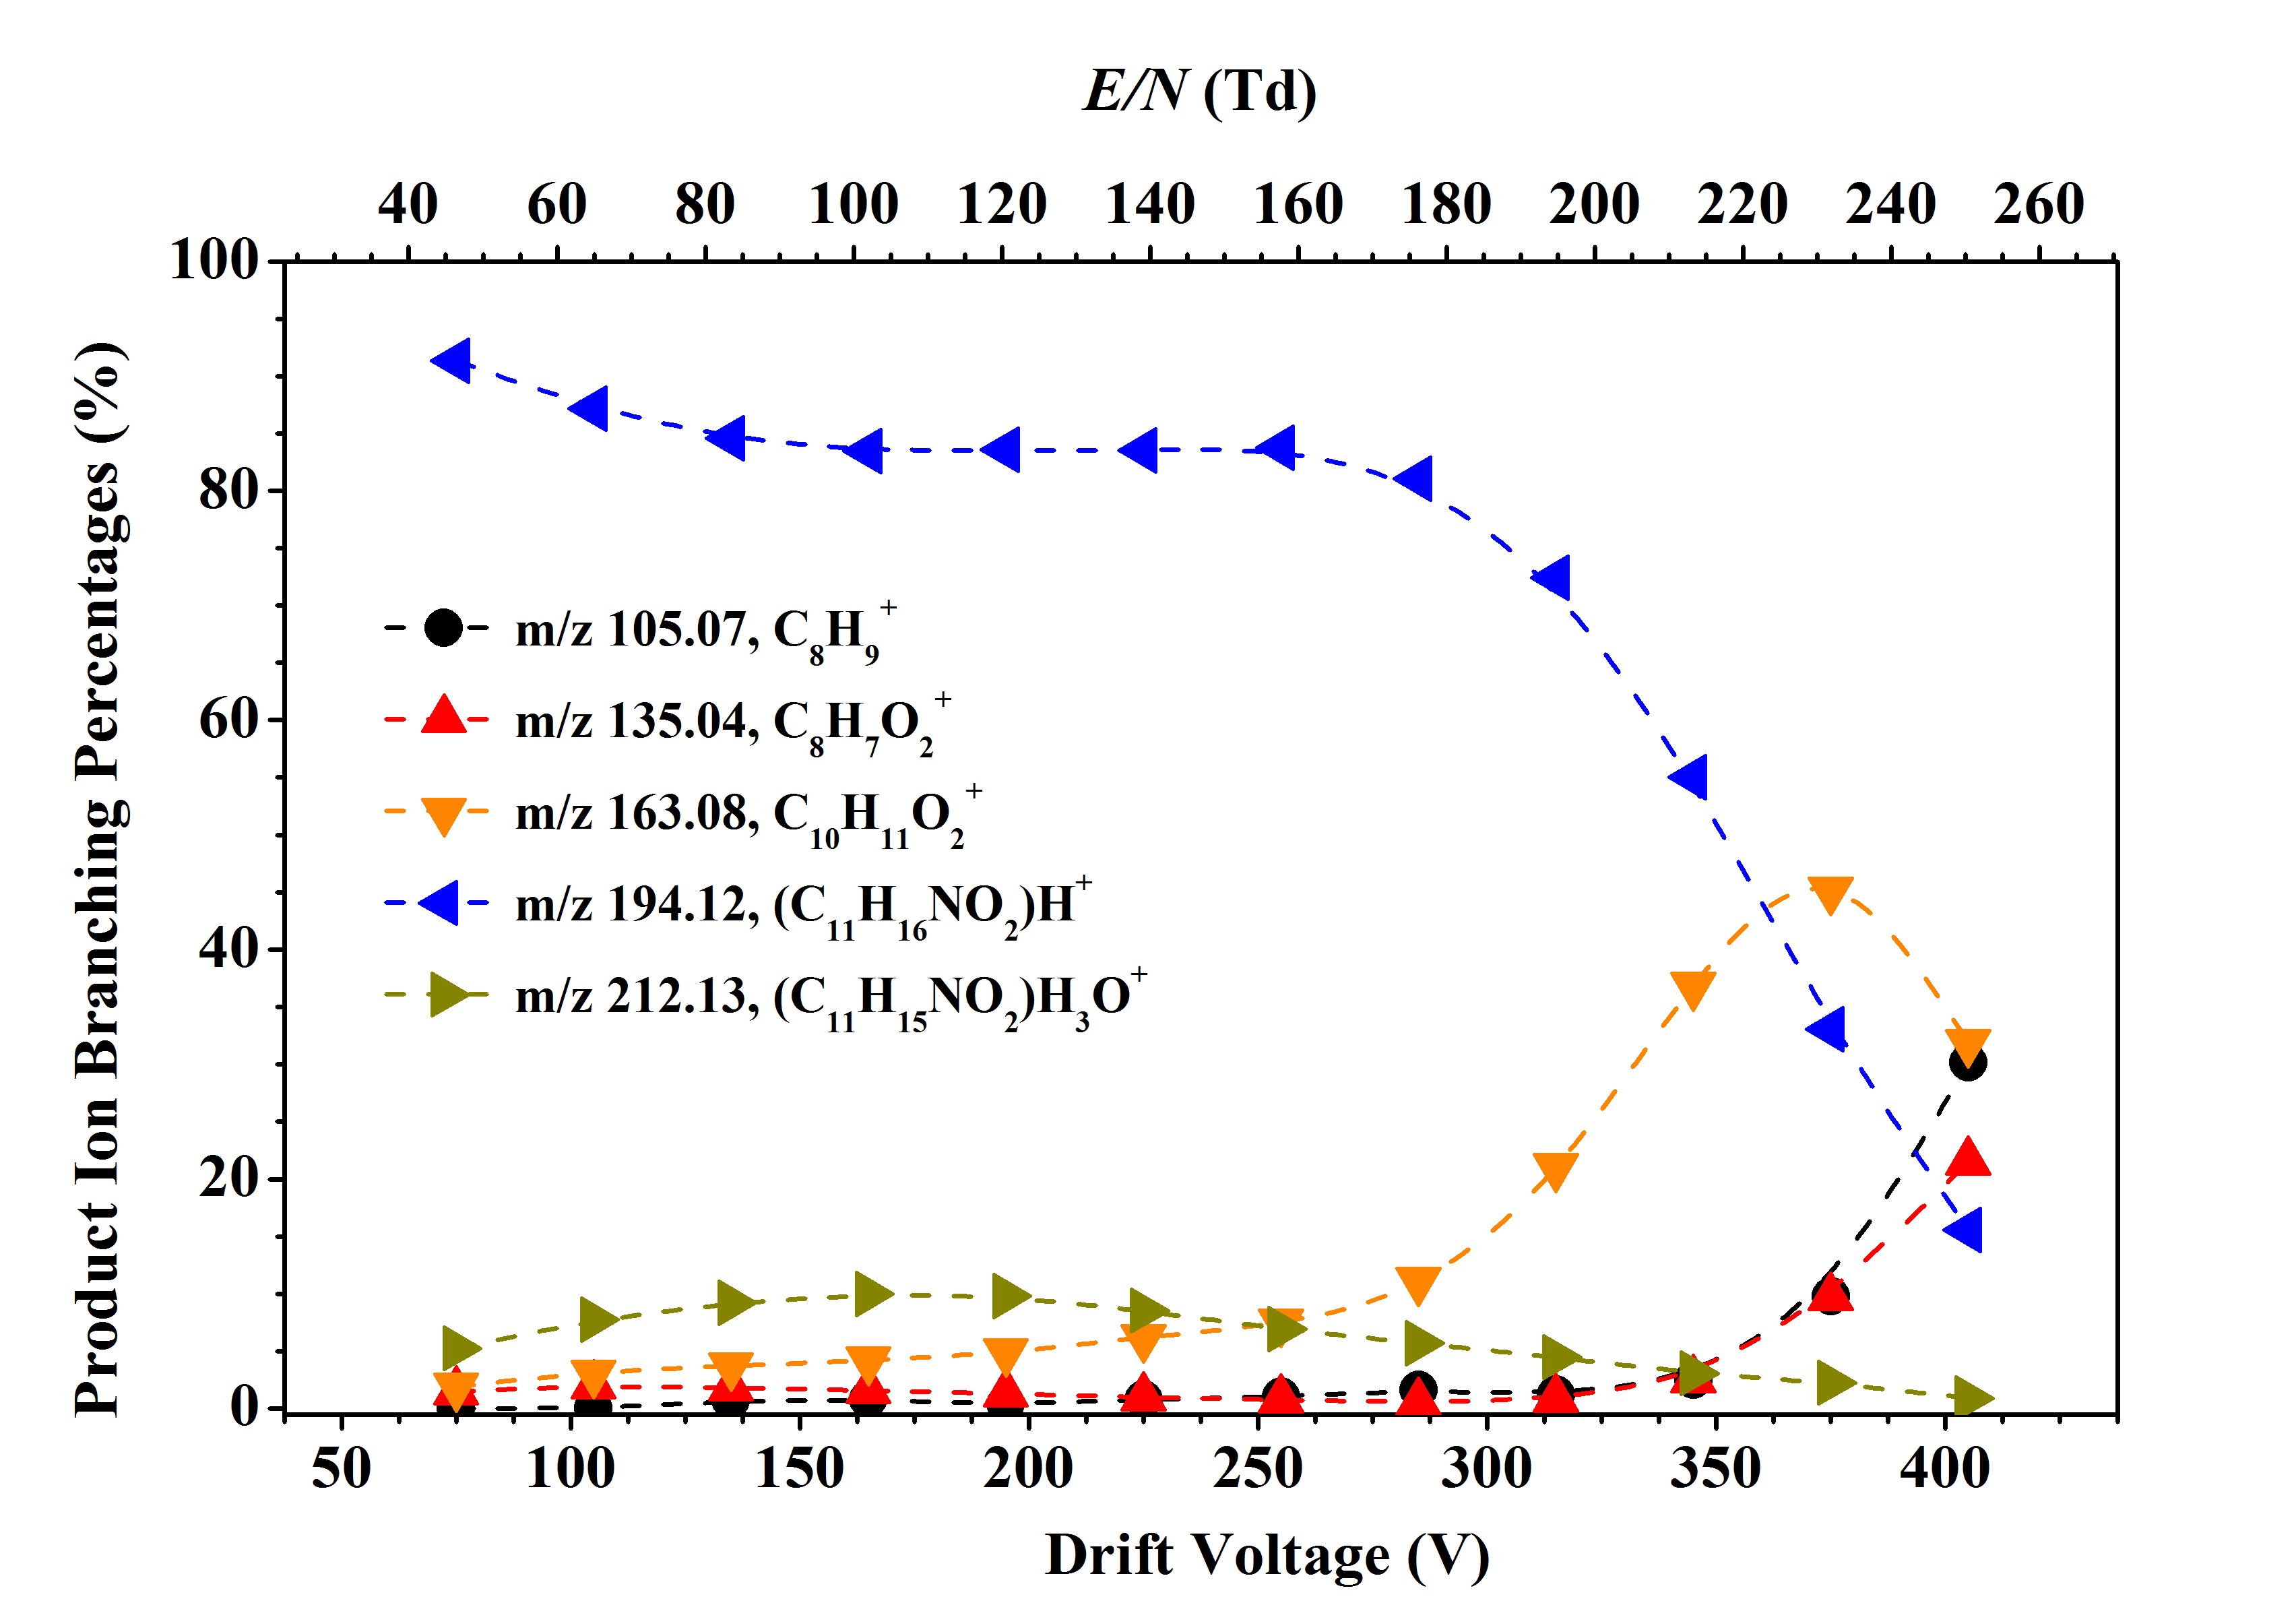
\includegraphics[width=0.80\linewidth]{pics/other_drugs/mdmaBRud.png}
\caption{Product ion distributions for MDMA as a function of the drift voltage and the reduced electric field.}
\label{fig:DR_mdma}
\end{figure}


\begin{figure}[htb]
\centering
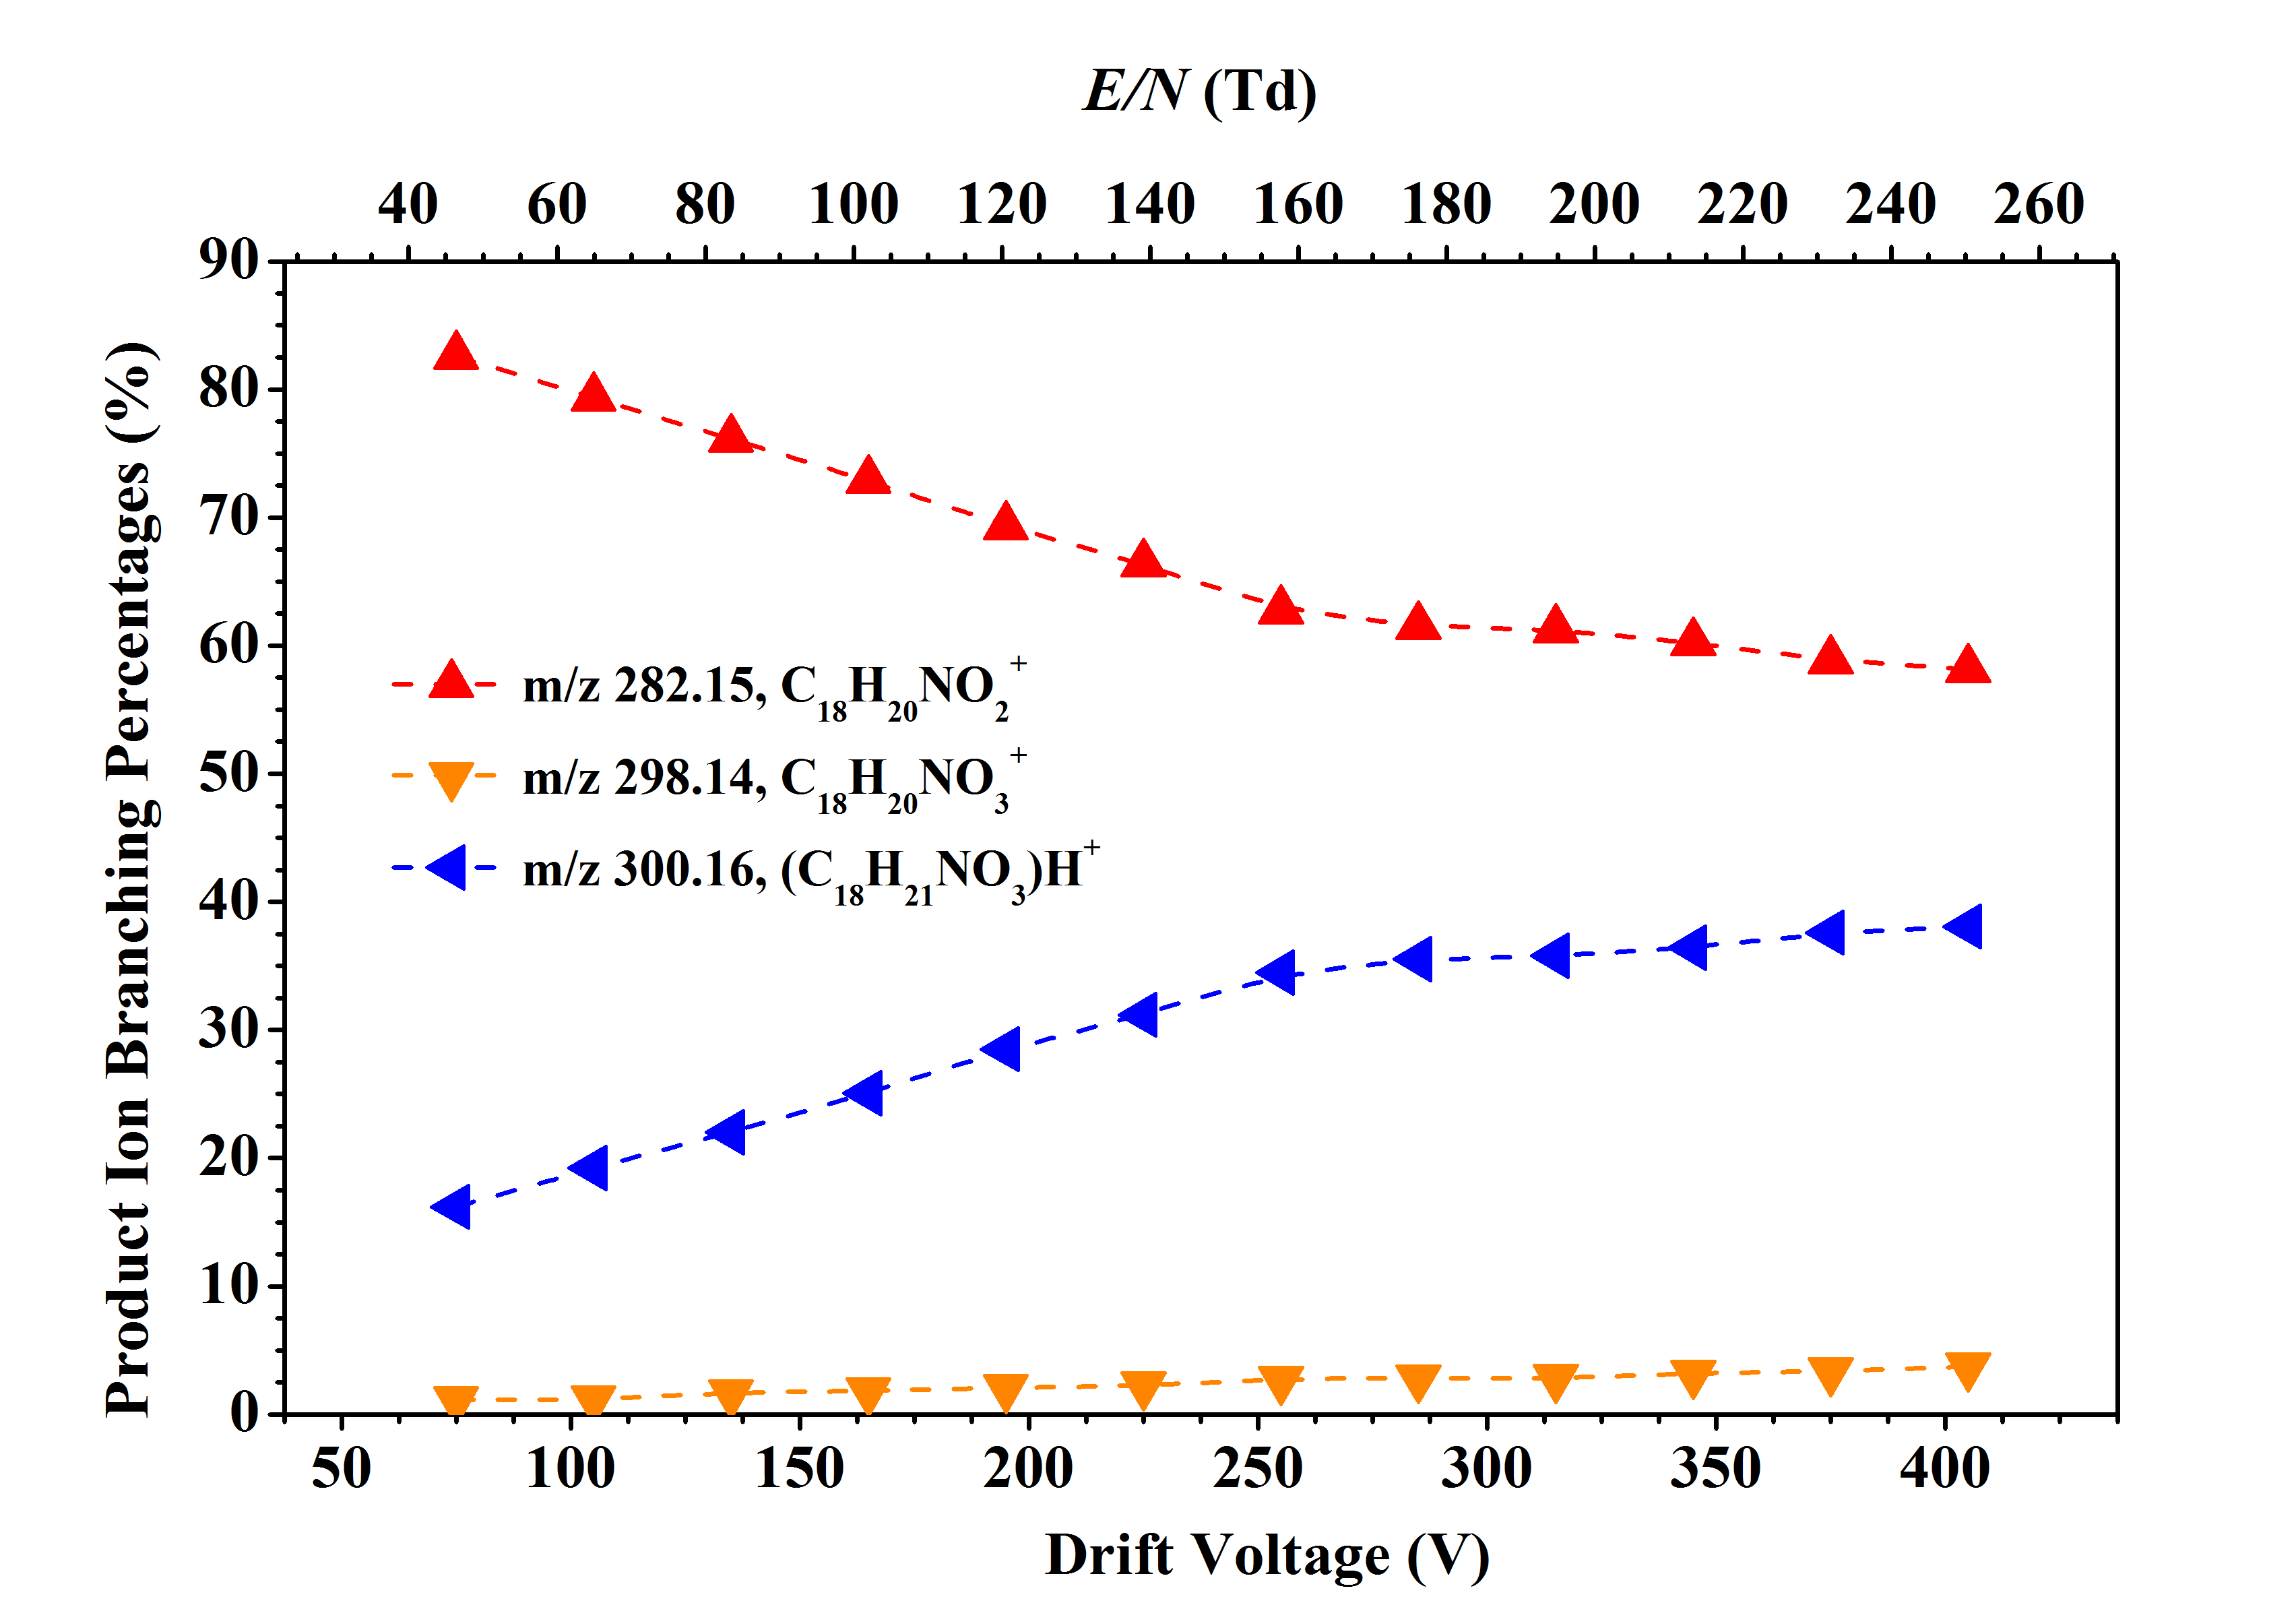
\includegraphics[width=0.80\linewidth]{pics/other_drugs/codeineBRud.png}
\caption{Product ion distributions for codeine as a function of the drift voltage and the reduced electric field.}
\label{fig:DR_codeine}
\end{figure}


\begin{figure}[htb]
\centering
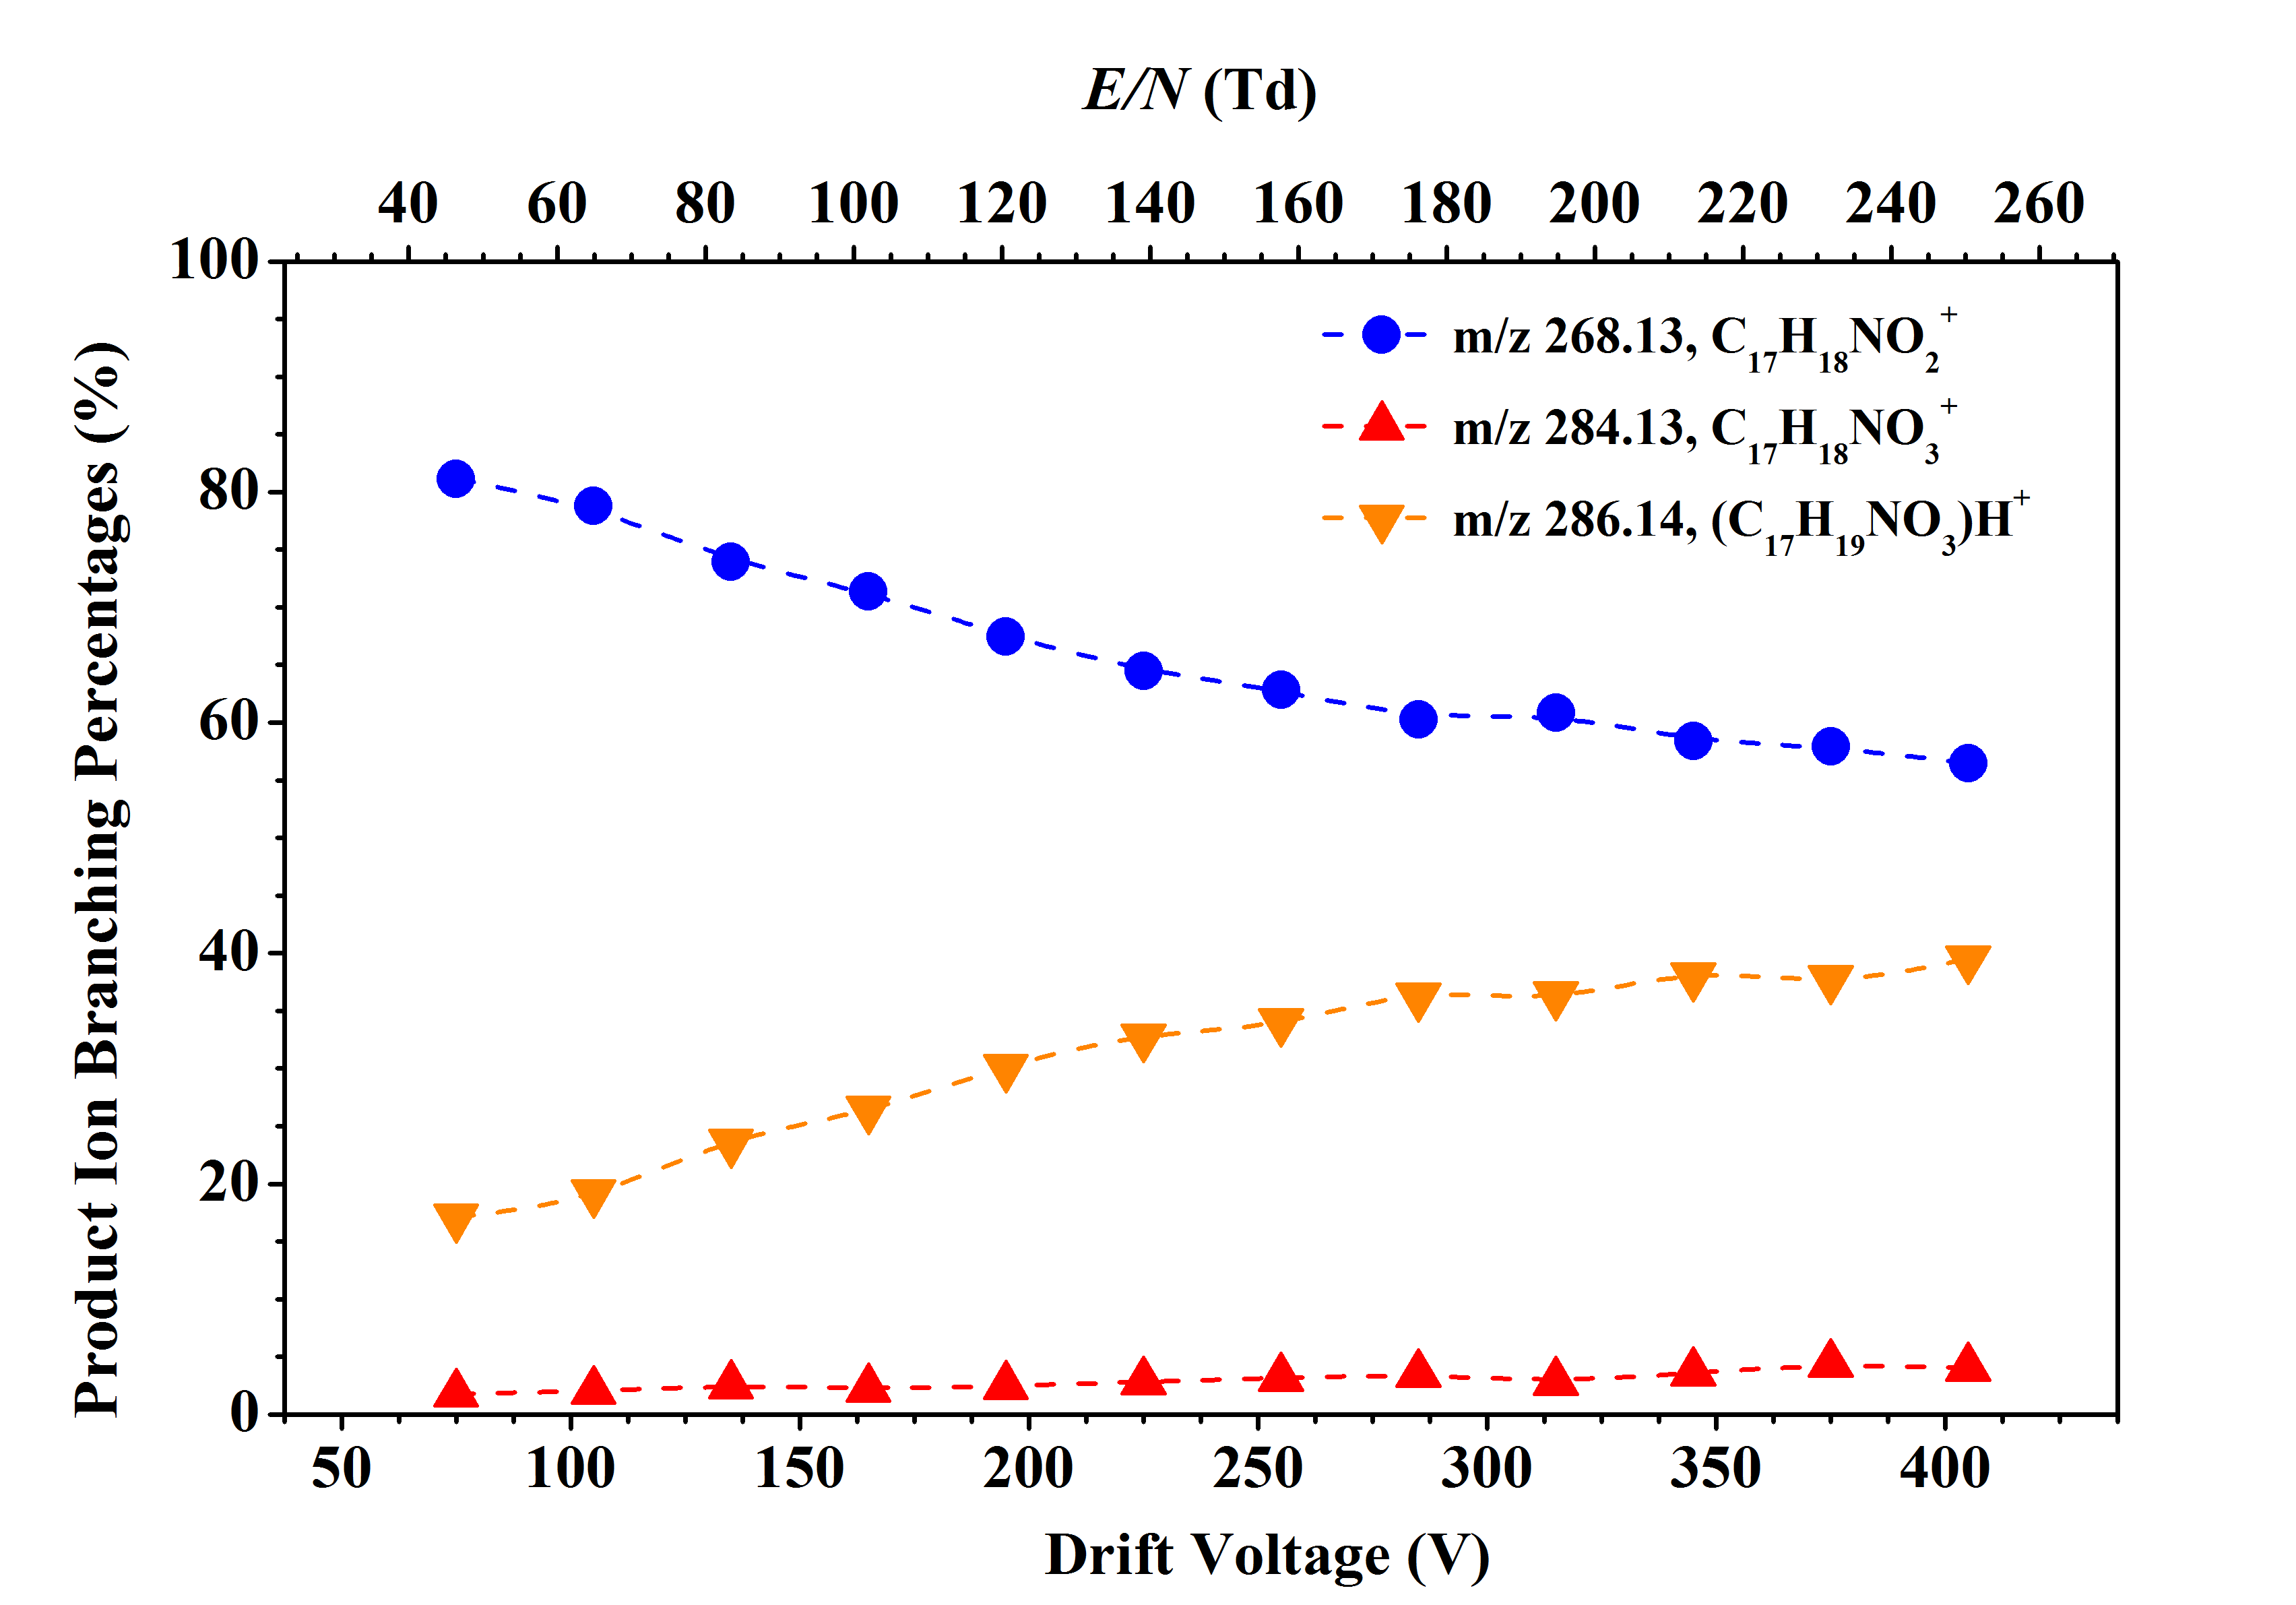
\includegraphics[width=0.80\linewidth]{pics/other_drugs/morphineBRud.png}
\caption{Product ion distributions for morphine as a function of the drift voltage and the reduced electric field.}
\label{fig:DR_morphine}
\end{figure}



%\subsubsection{Ethanol}

%This measurement was done to study the loss of H$_2$ in alcohols -- it happens in morphine, heroin, etc.\textbf{INclude figure!!!!!!!!}


\begin{figure}[htb]
\centering
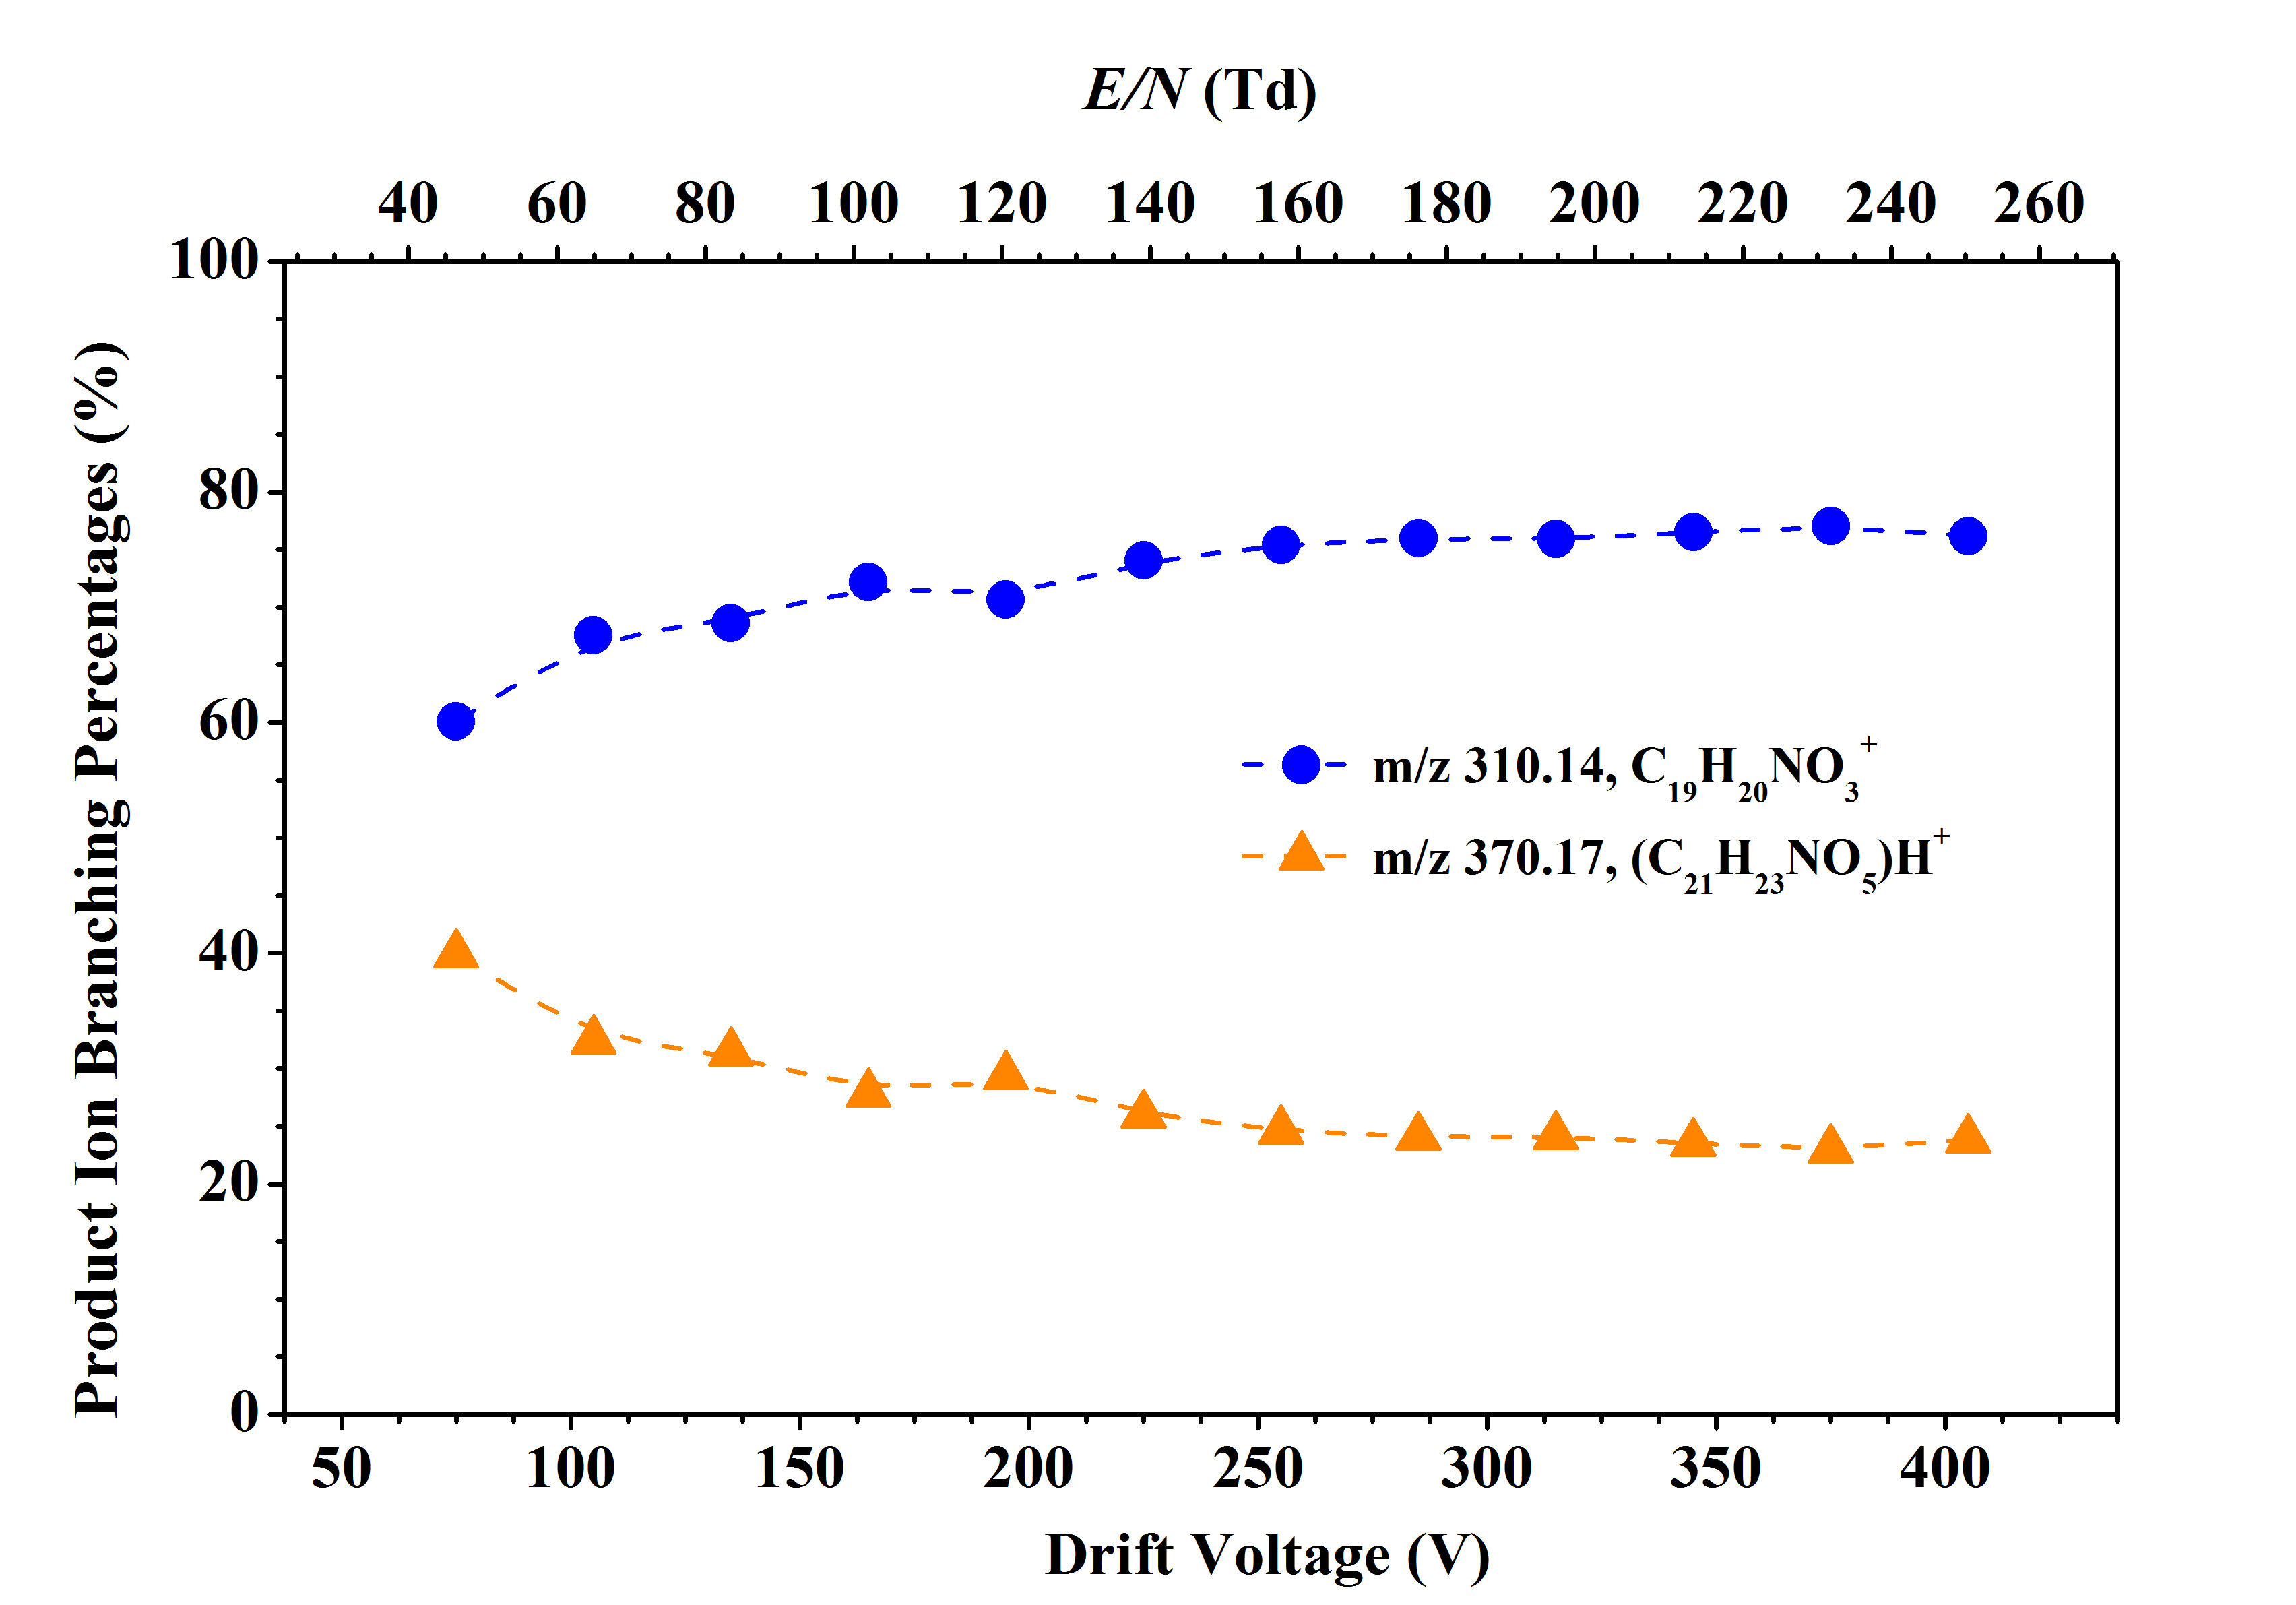
\includegraphics[width=0.80\linewidth]{pics/other_drugs/heroinBRud.png}
\caption{Product ion distributions for heroin as a function of the drift voltage and the reduced electric field.}
\label{fig:DR_CBN}
\end{figure}





\begin{figure}[htb]
\centering
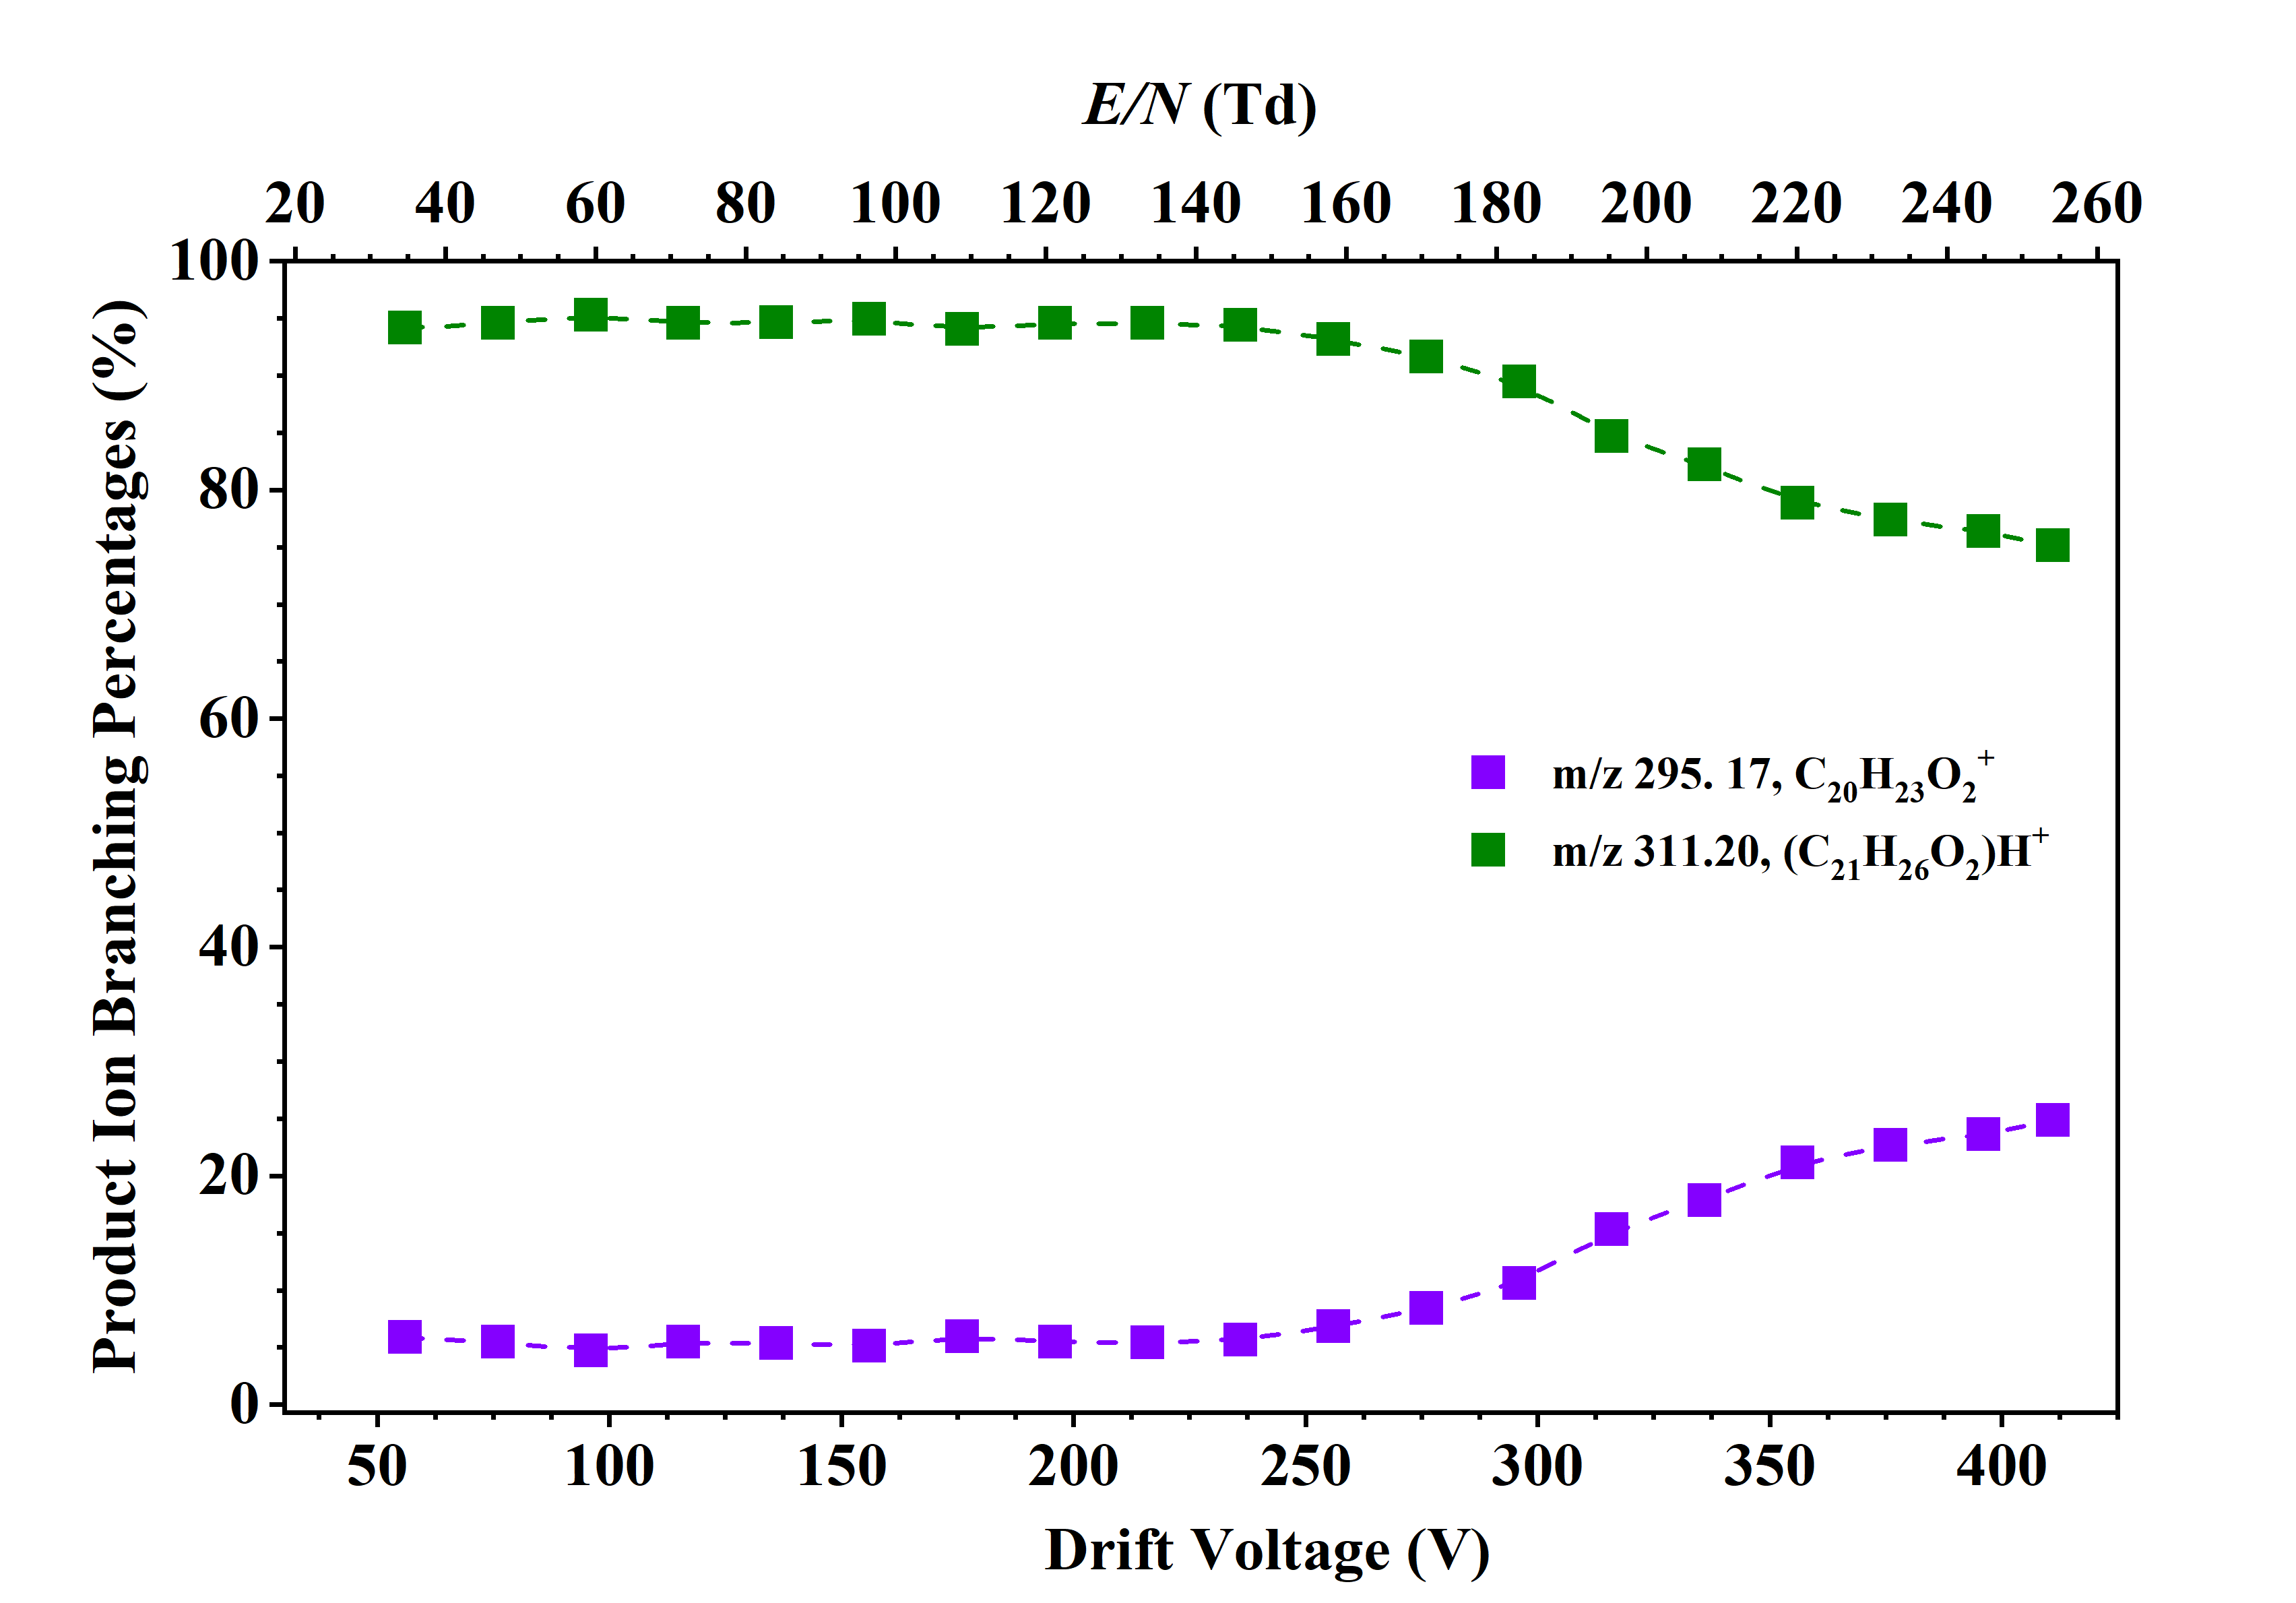
\includegraphics[width=0.80\linewidth]{pics/other_drugs/CBN-br.png}
\caption{Product ion distributions for CBN as a function of the drift voltage and the reduced electric field.}
\label{fig:DR_CBN}
\end{figure}

 
\begin{figure}[htb]
\centering
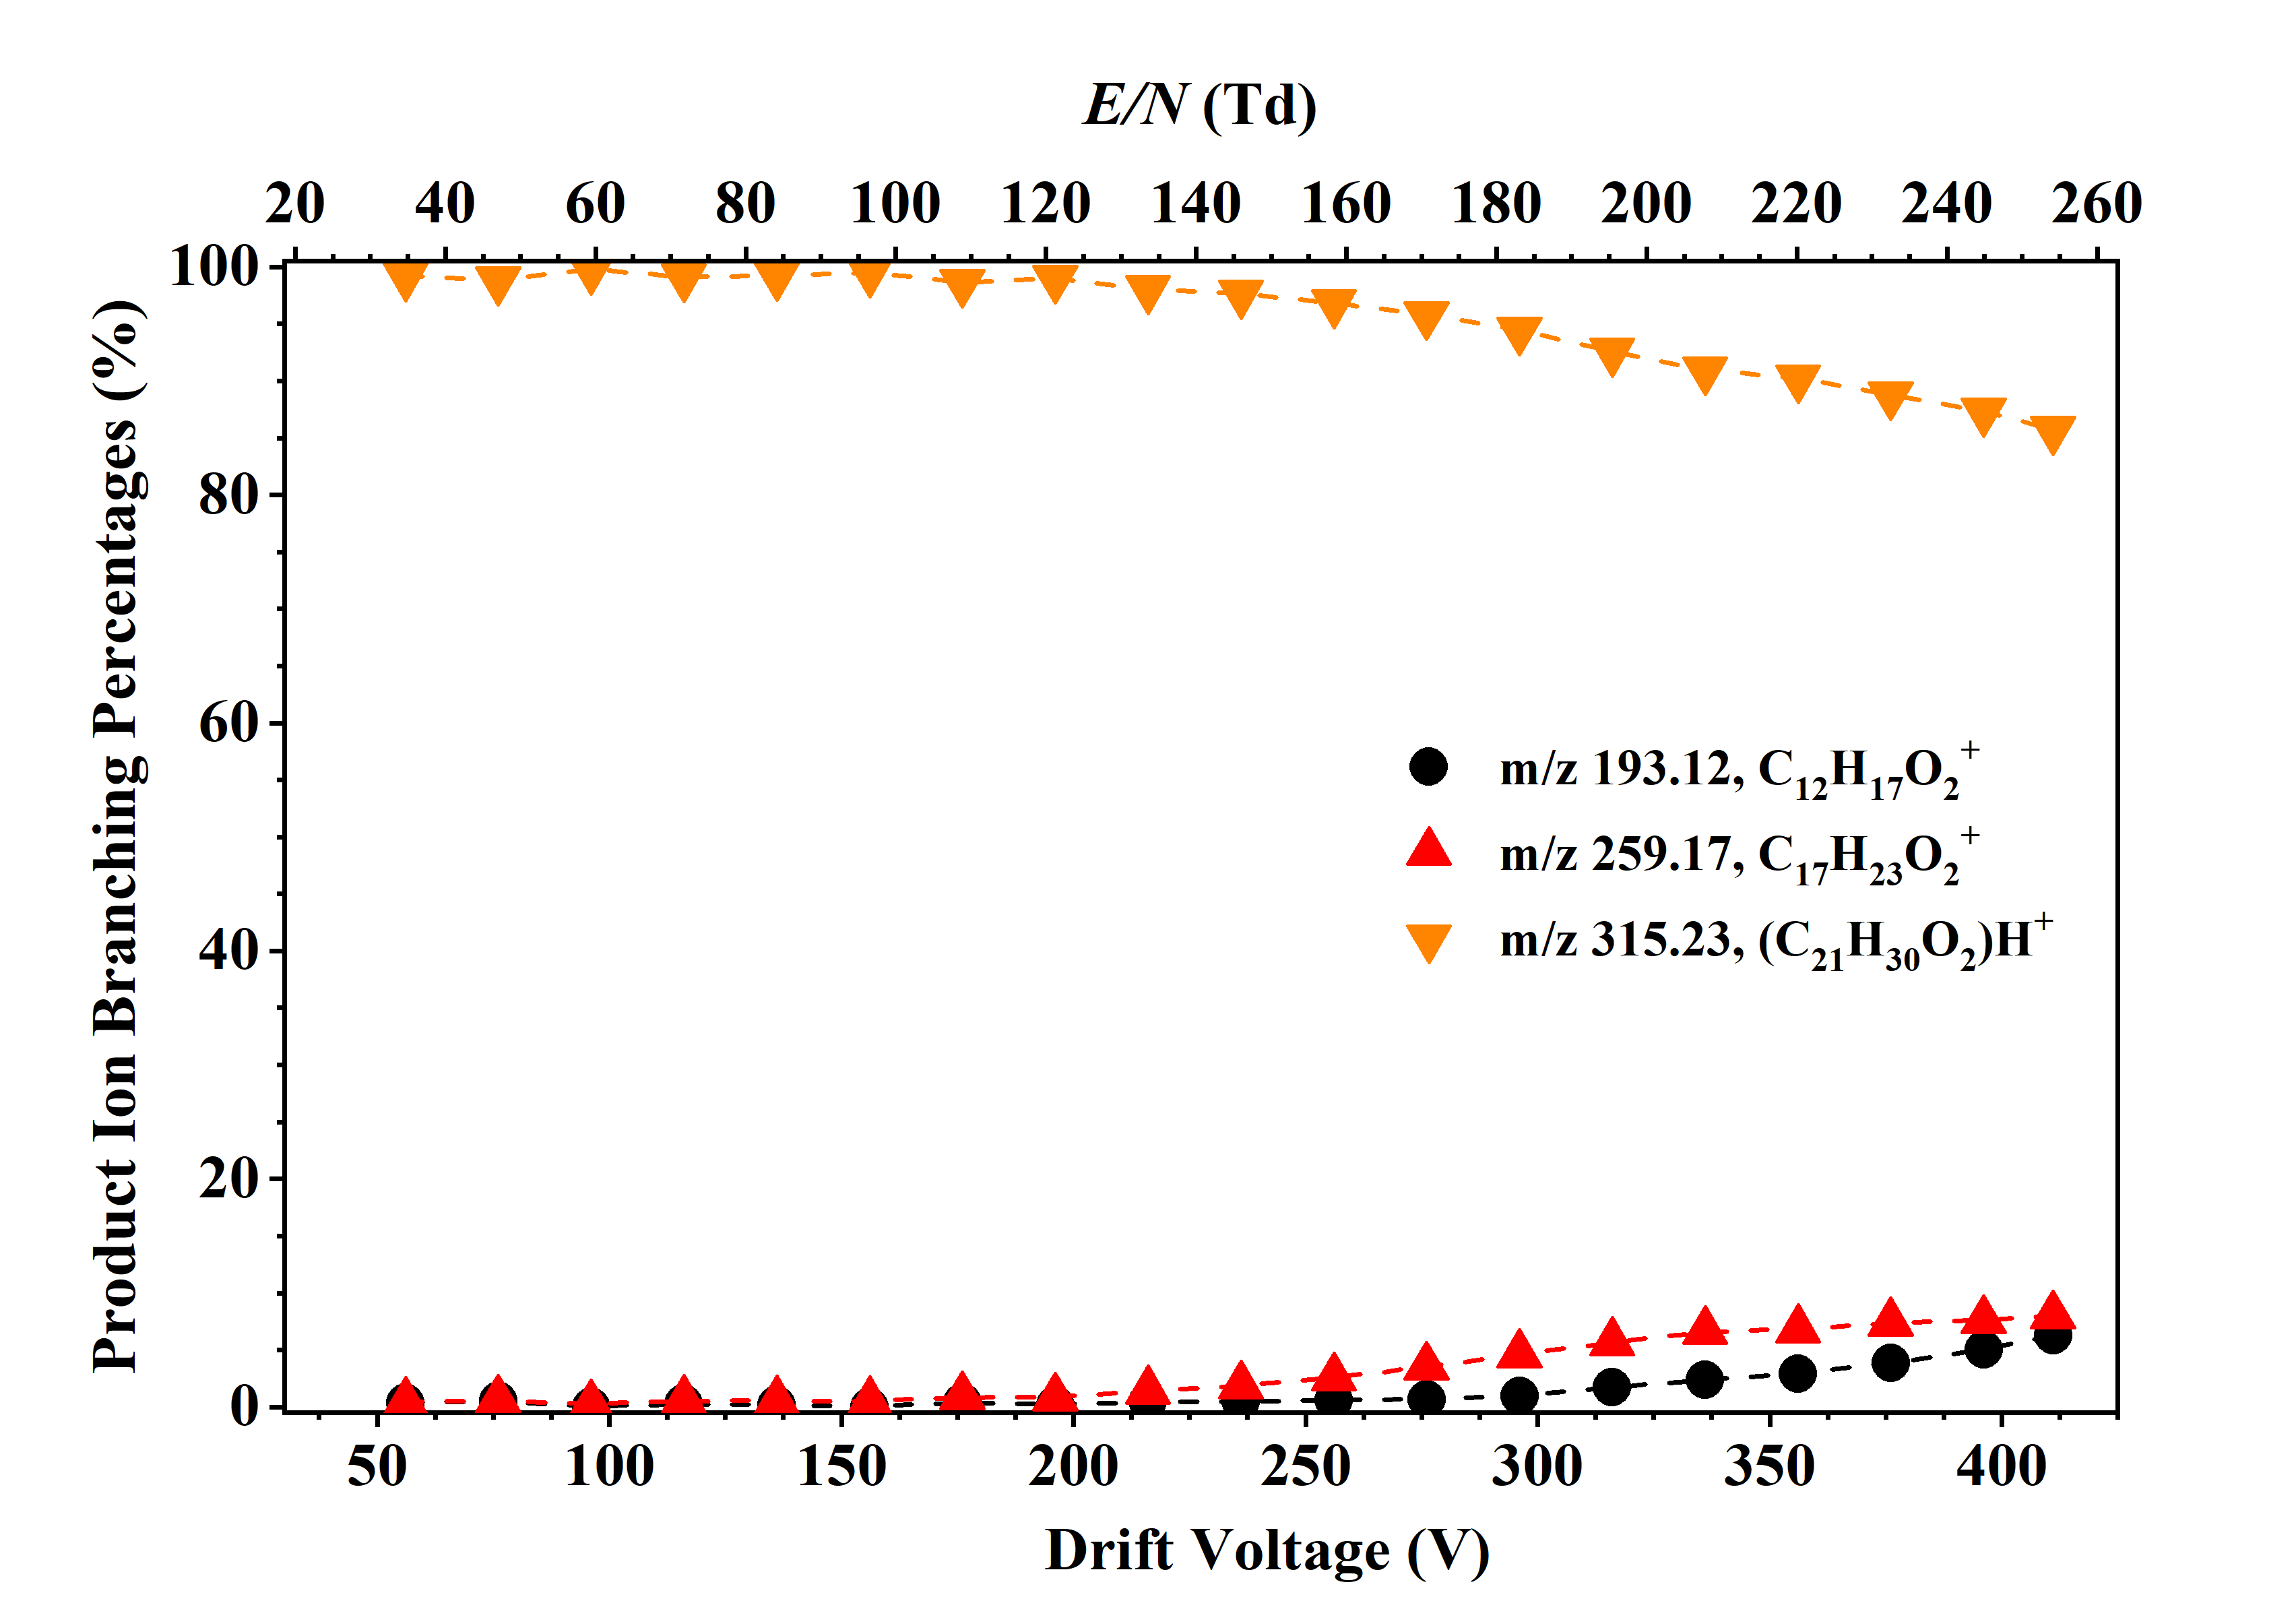
\includegraphics[width=0.80\linewidth]{pics/other_drugs/THC-br.png}
\caption{Product ion distributions for $\Delta$-9-THC as a function of the drift voltage and the reduced electric field.}
\label{fig:DR_THC}
\end{figure}



\begin{figure}[htb]
\centering
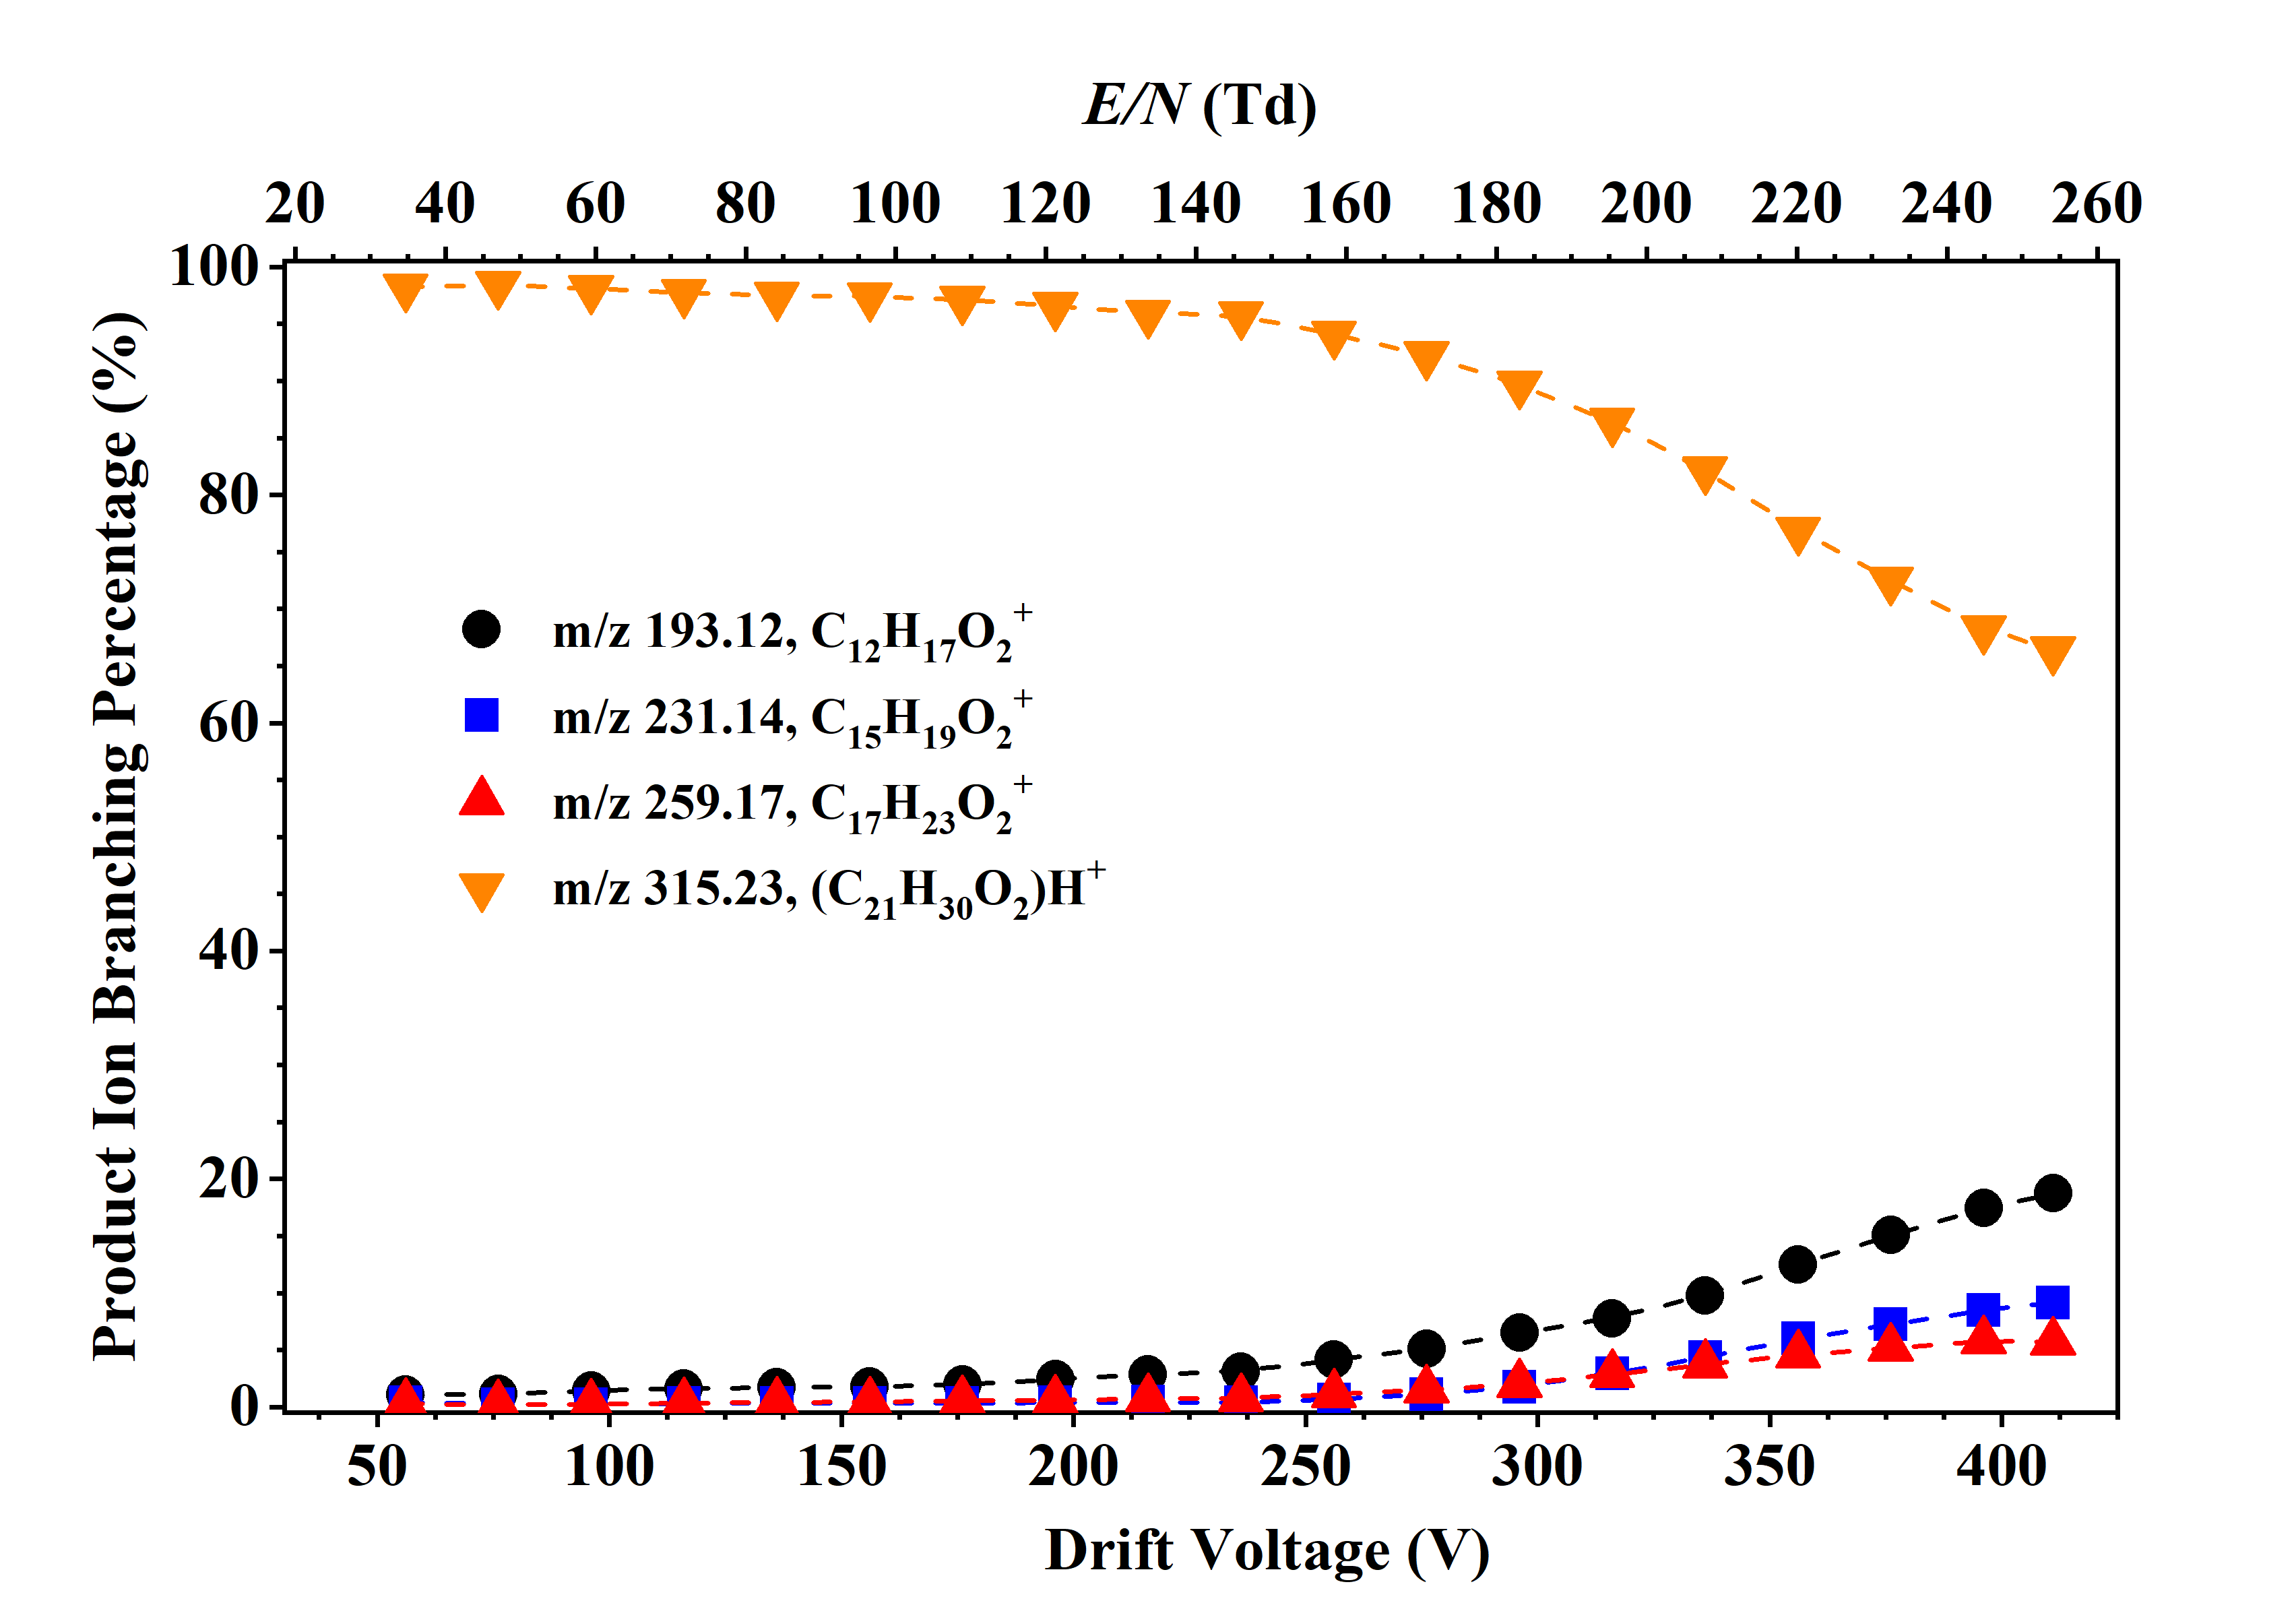
\includegraphics[width=0.80\linewidth]{pics/other_drugs/CBD-br.png}
\caption{Product ion distributions for CBD as a function of the drift voltage and the reduced electric field.}
\label{fig:DR_CBD}
\end{figure}


% to separate sections
%\FloatBarrier

%%%%%%%%%%%%%%%%%%%%%%%%%%%%%%%%%%%%%%%%%%%%%%%%%%%%%%%%%%%%%%%%%%%%%%%%%%%%%%%%%%%%%%%%%%%%%%%%%%%%%%%%%%%%%%%%%%%%%%%%%%%%%%%%%%%%%%%%%%%%%%%%%%%%%%%%%%%%%%%%%%%%%%%%%%%%%%%%%%%%%%%%%%%%%%%%%%%%%%%%%%%%%%%%%%5
\section{Reduced electric field fast switching results}
The \textit{E/N} fast switching results presented here have been averaged over each cycle.
%
The switching frequency is 1 Hz for all the experiments.
%
%Shown in figures (>>>>>>>>>>>). Reagent ion shown in ...........
%
This section includes fast switching results of 
(H$_2$O)$_n$H$_3$O$^+$ (n = 0, 1) (\autoref{fig:DR_RI_fs}), 
cocaine (\autoref{fig:DR_COC_fs}),
methyl ecgonine (\autoref{fig:DR_MeEcg_fs}),
ethyl ecgonine (\autoref{fig:DR_EtEcg_fs}),
norcocaine (\autoref{fig:DR_norcocaine_fs}),
o-hydroxycocaine (\autoref{fig:DR_ohcocaine_fs}),
CBN (\autoref{fig:DR_CBN_fs}),
$\Delta$-9-THC (\autoref{fig:DR_THC_fs})
and
CBD (\autoref{fig:DR_CBD_fs}).



\begin{figure}[htb]
\centering
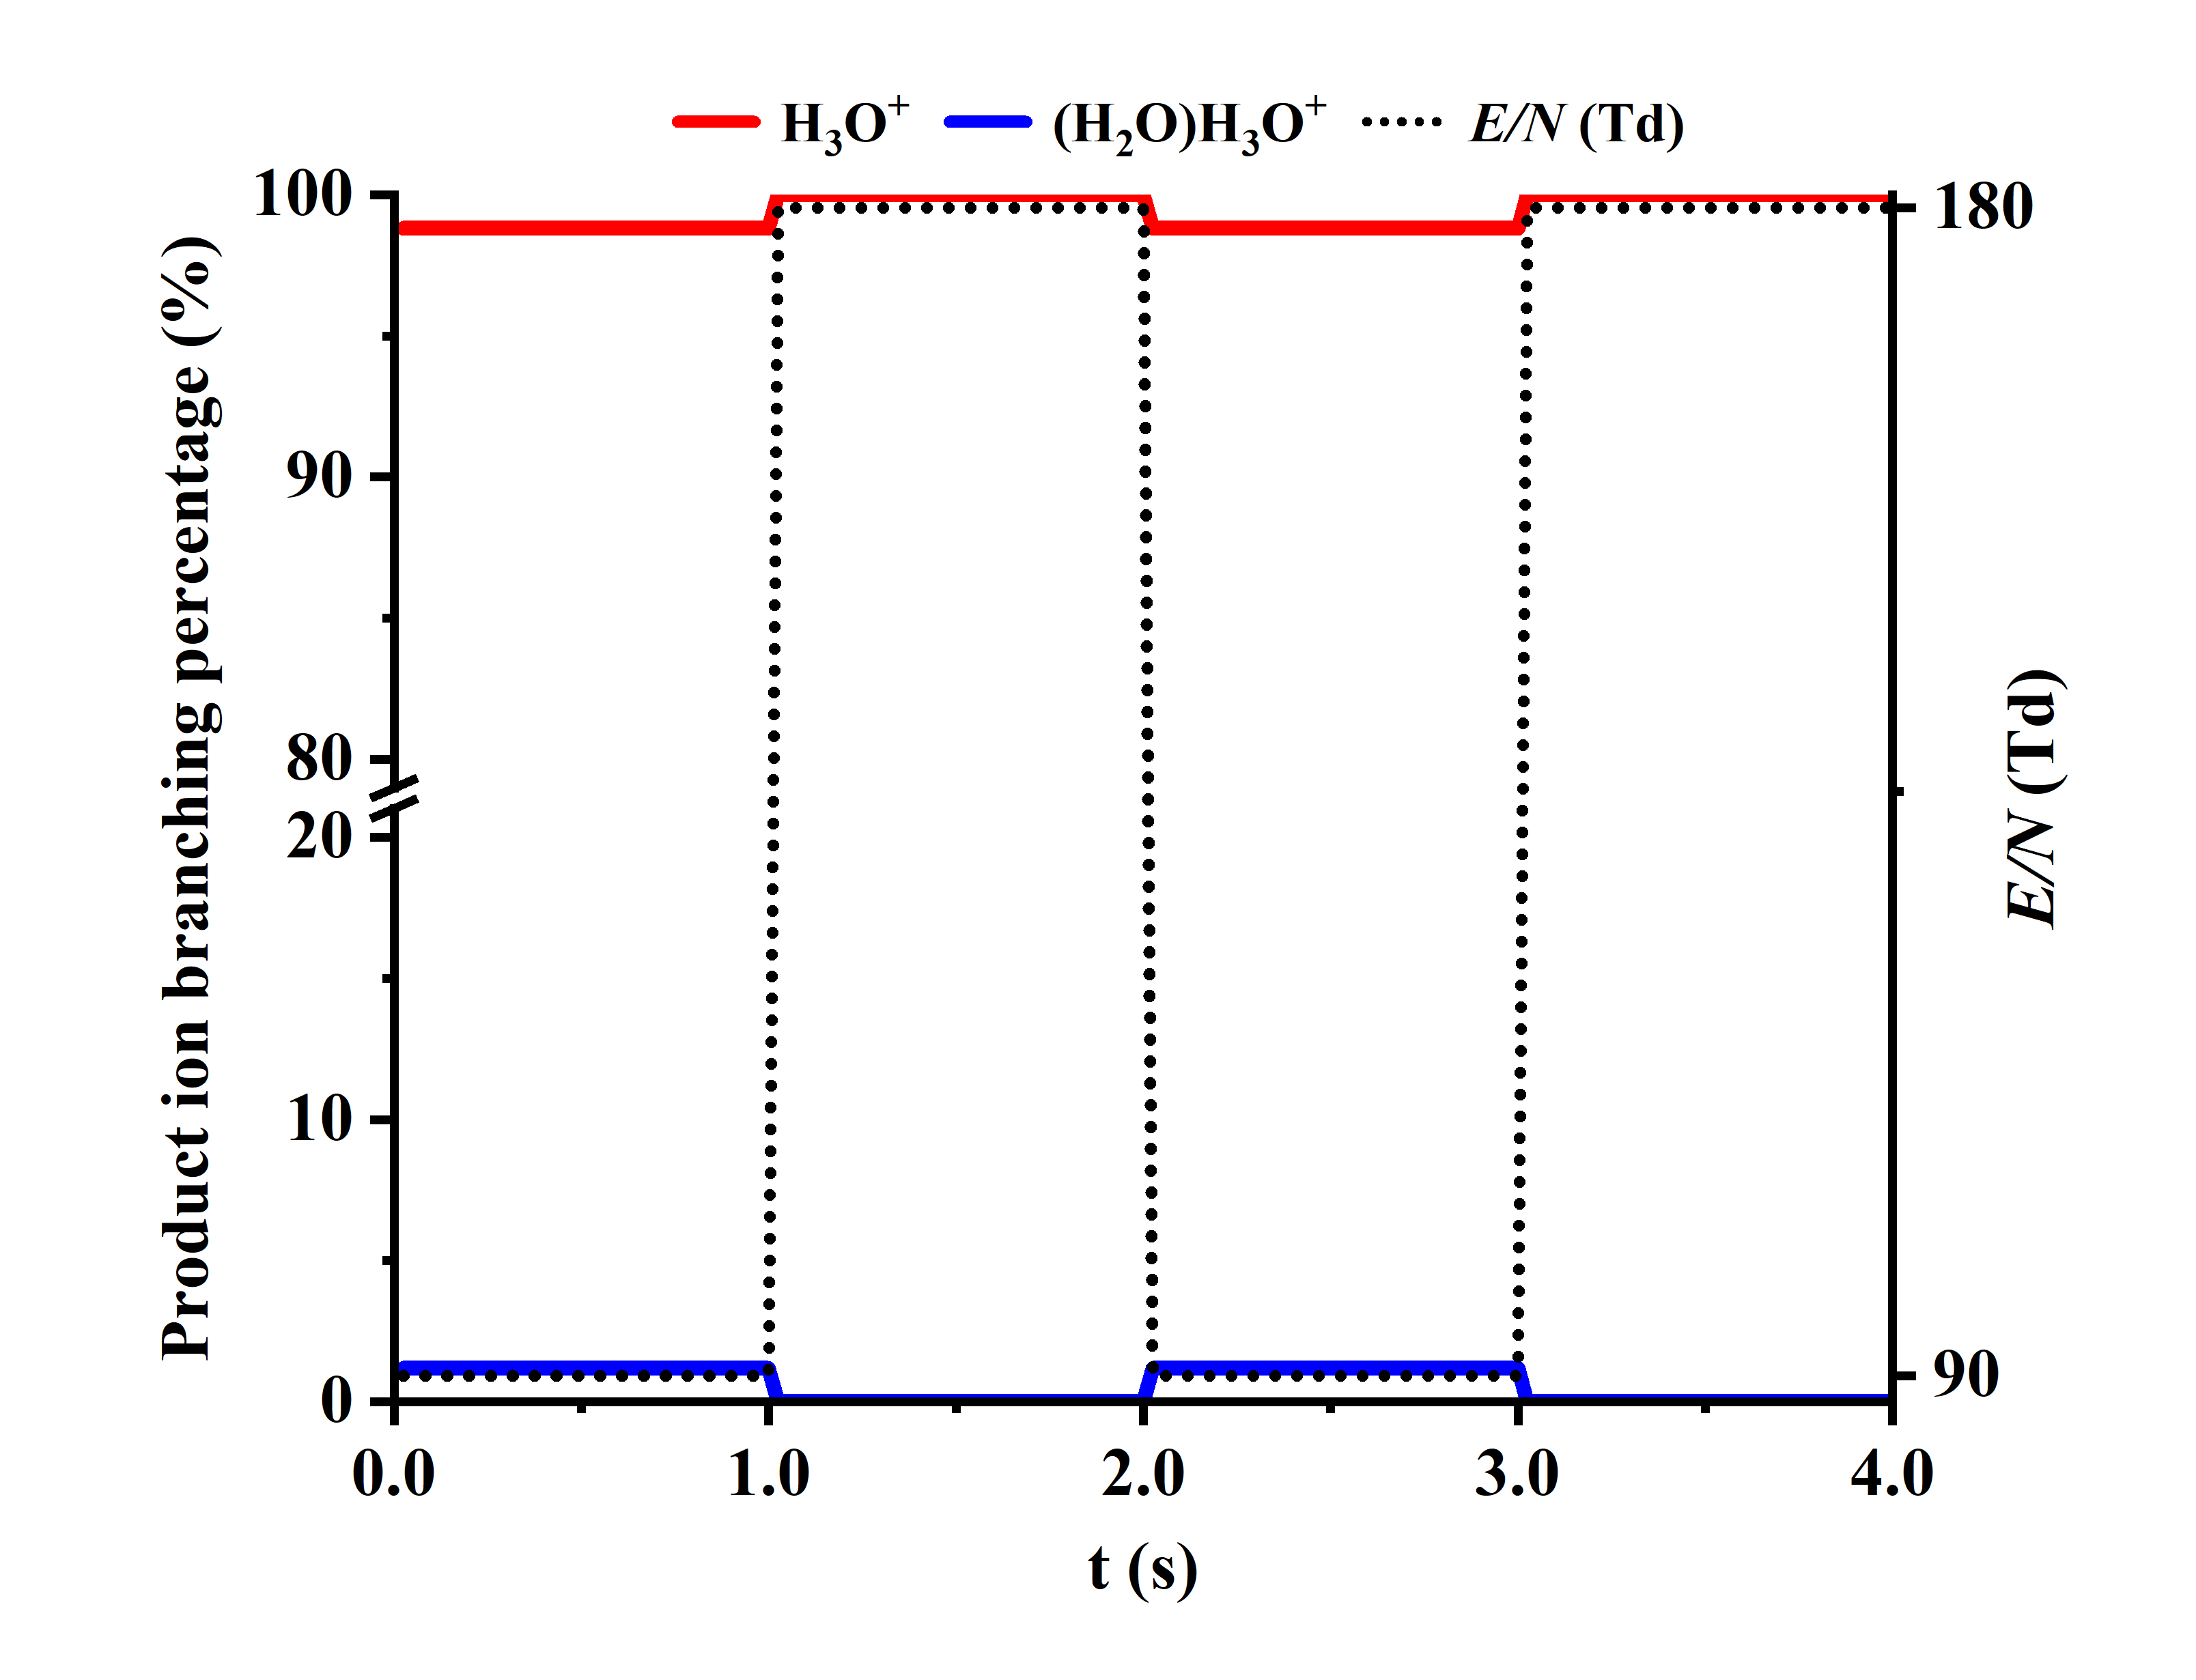
\includegraphics[width=0.80\linewidth]{pics/RIDPM90180Td-averaged.png}
\caption{Reagent ions reduced electric field fast switching plot.}
\label{fig:DR_RI_fs}
\end{figure}


\begin{figure}[htb]
\centering
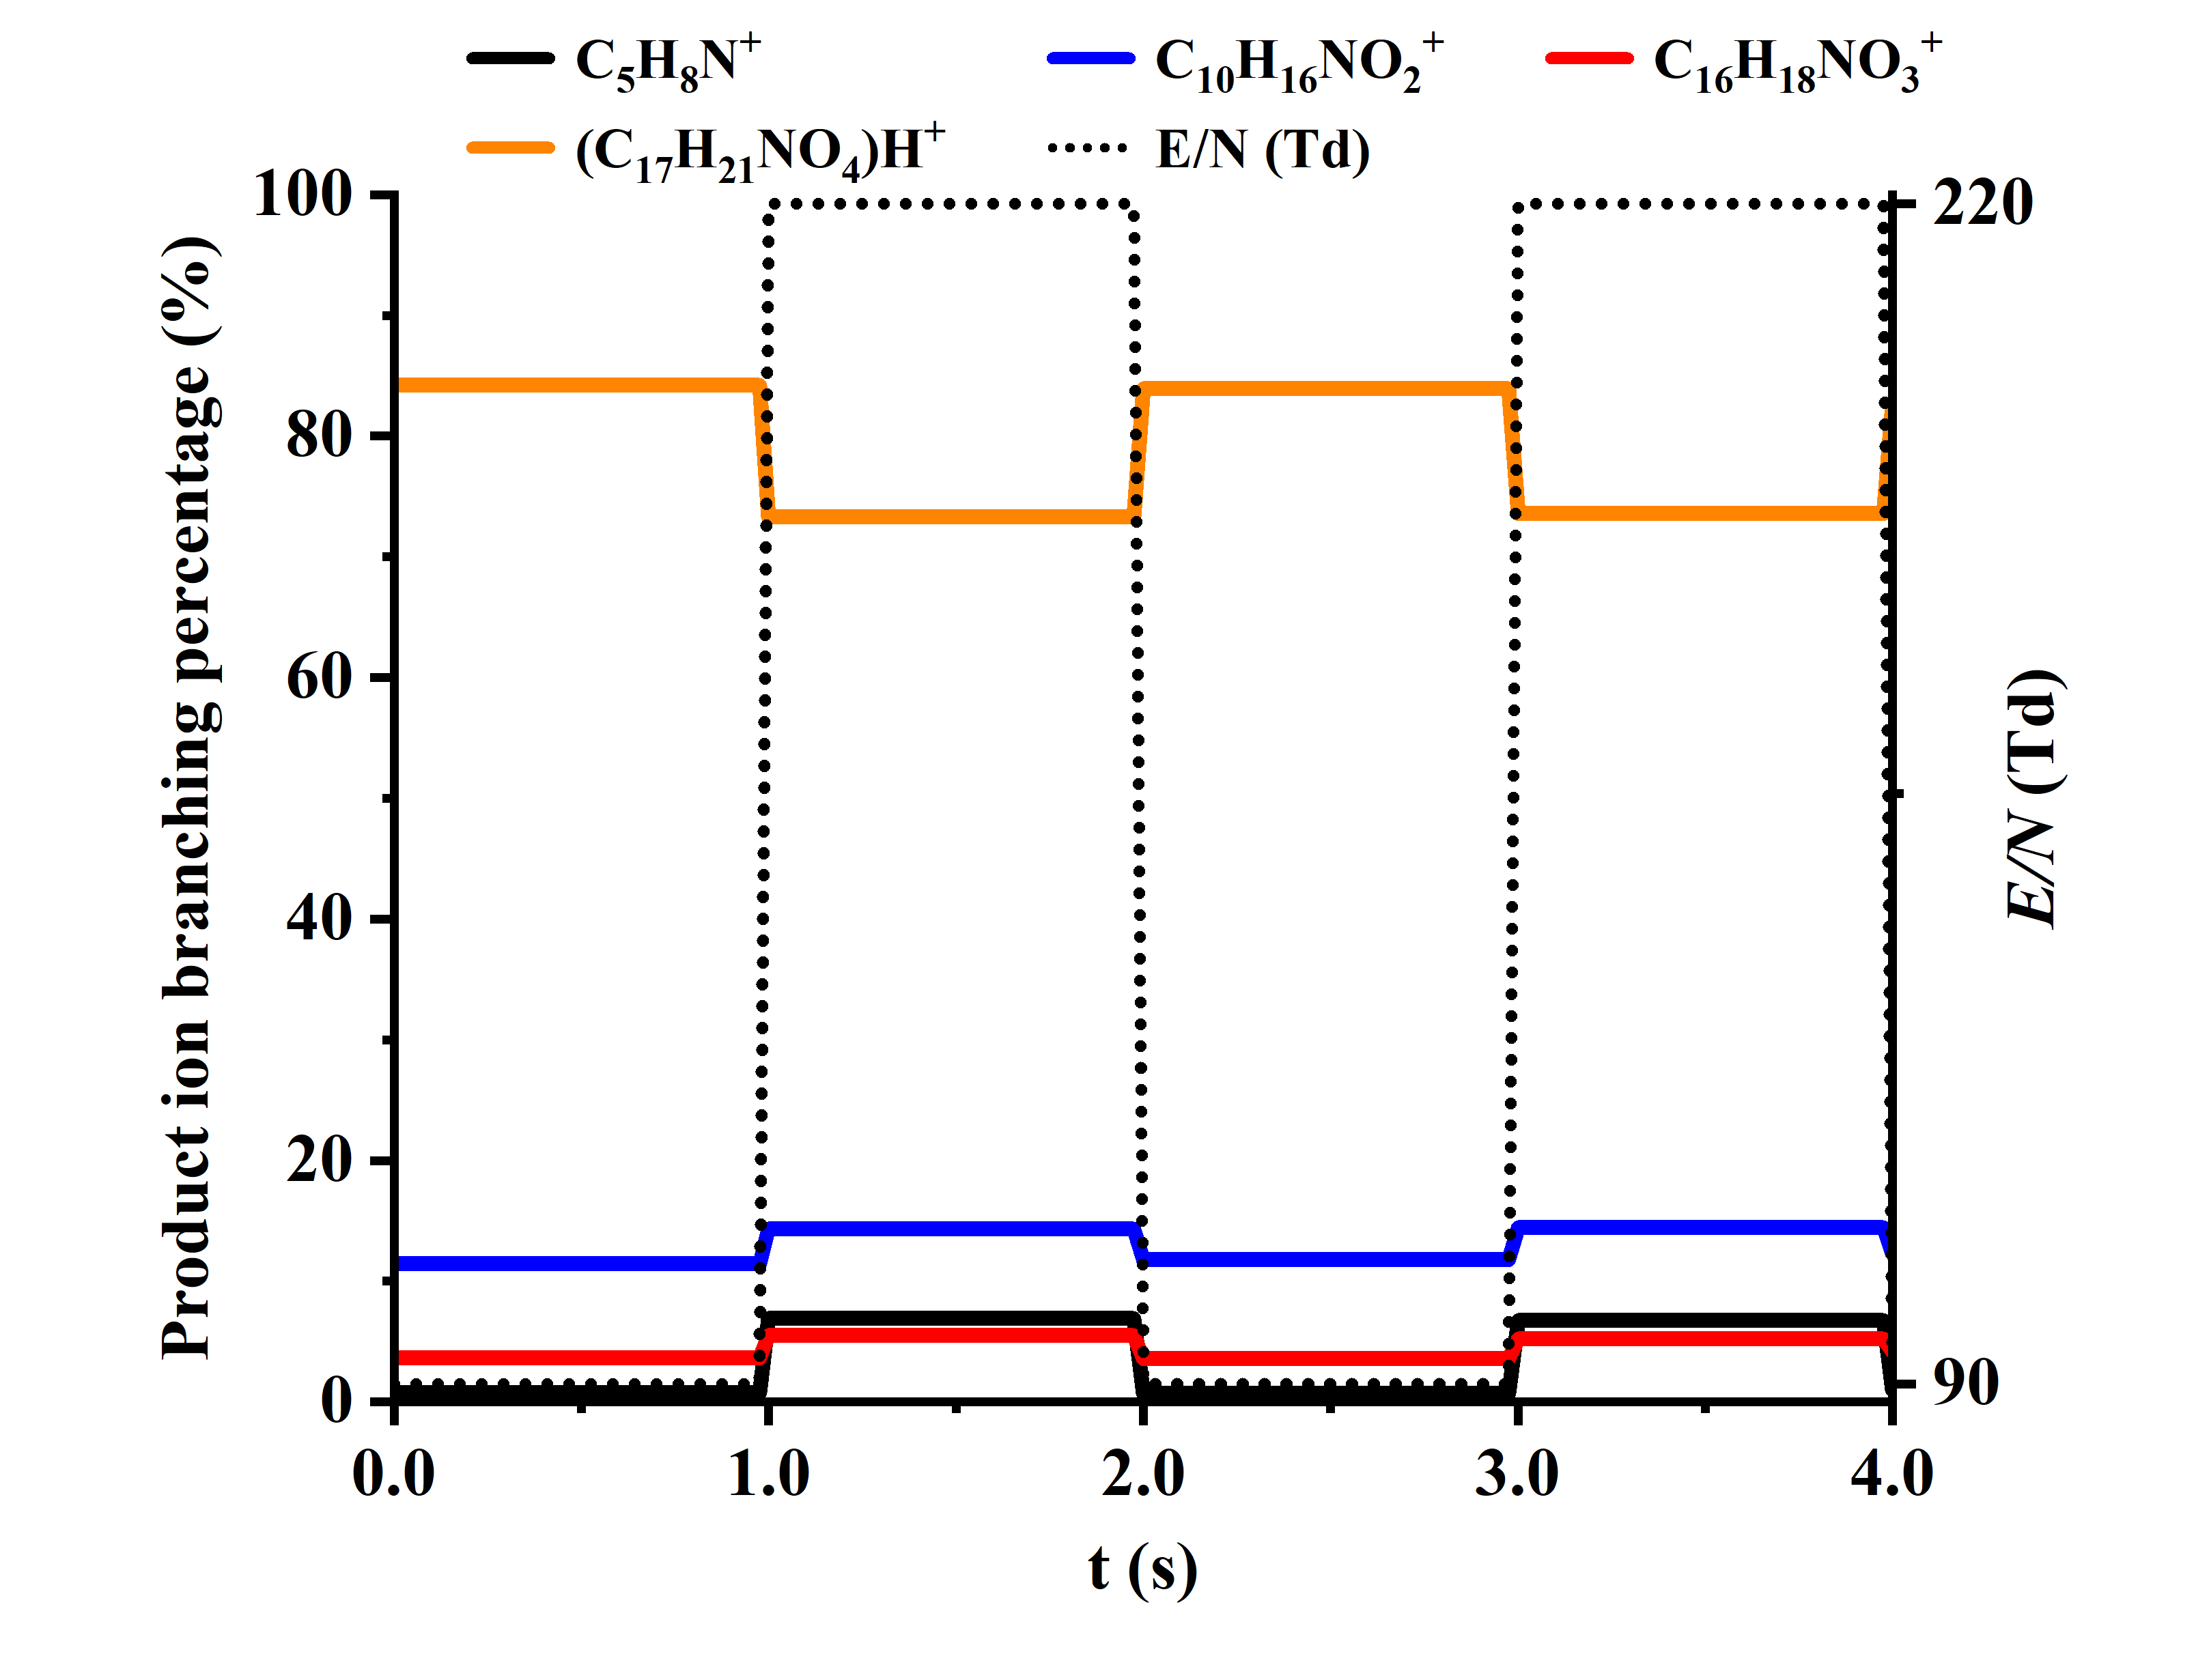
\includegraphics[width=0.80\linewidth]{pics/other_drugs/coc-fs-90-220.png}
\caption{Cocaine reduced electric field fast switching plot.}
\label{fig:DR_COC_fs}
\end{figure}



\begin{figure}[htb]
\centering
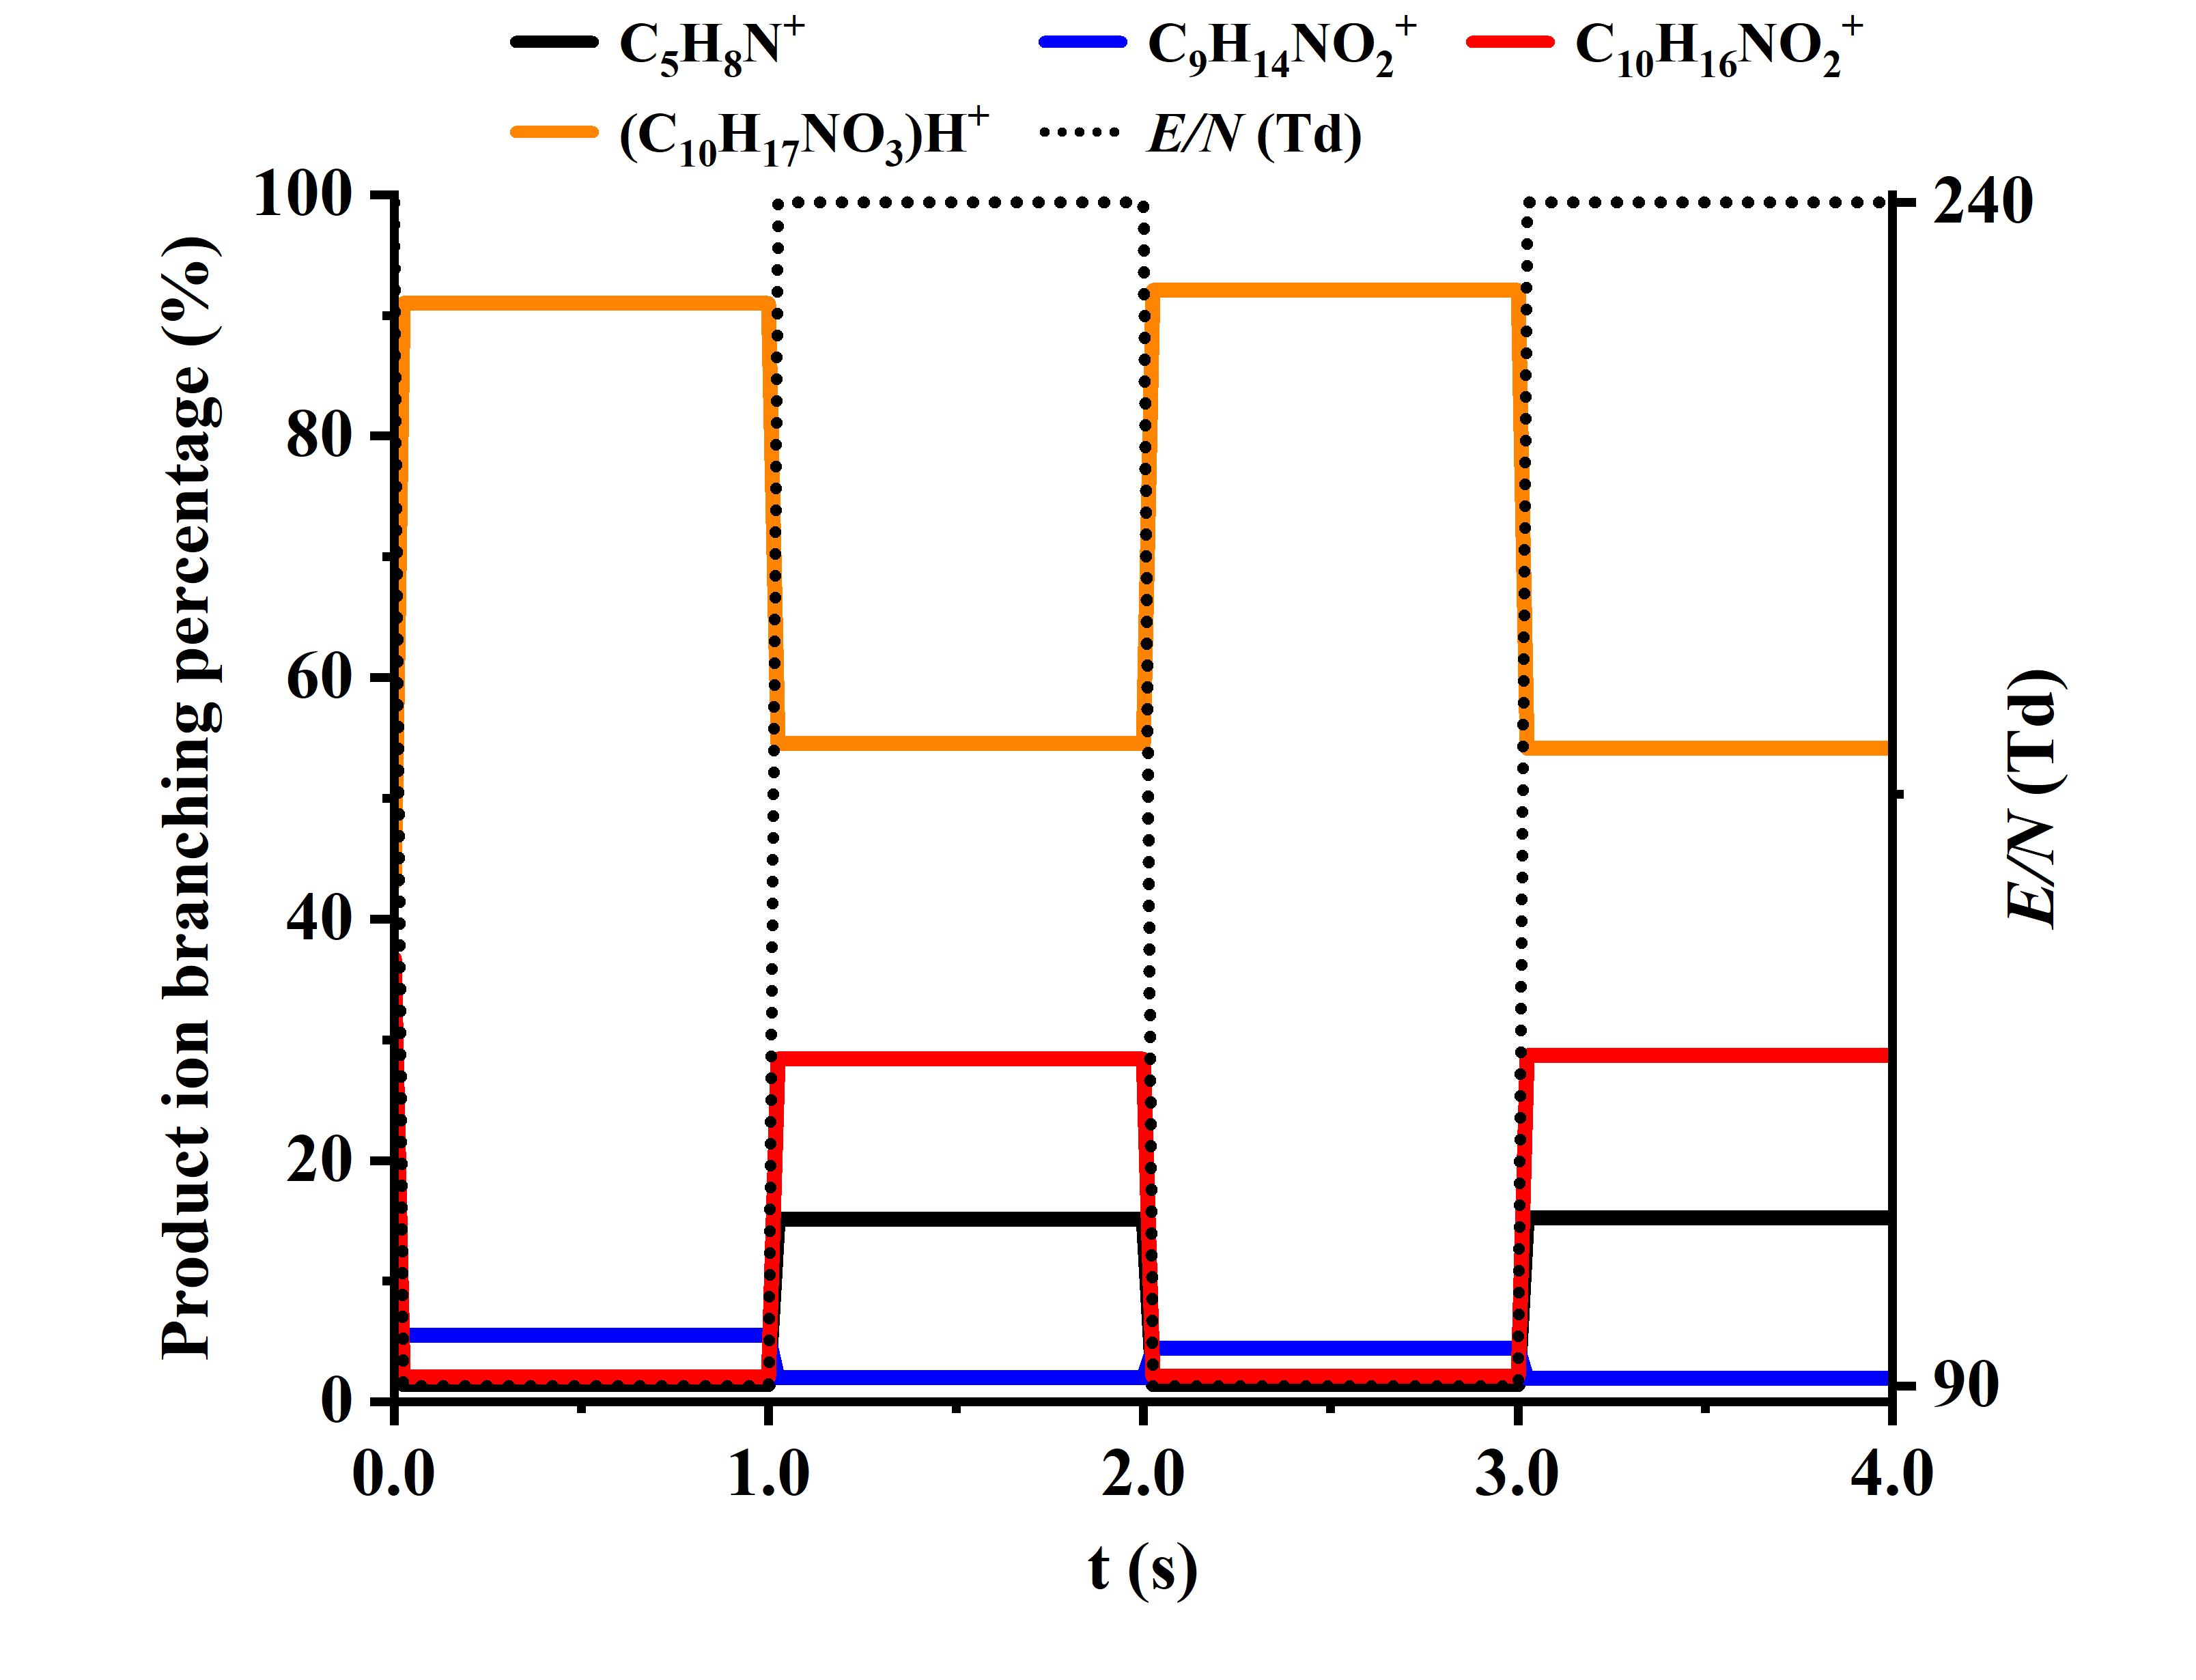
\includegraphics[width=0.80\linewidth]{pics/other_drugs/MeEcg-fs-90-240.png}
\caption{Methyl ecgonine reduced electric field fast switching plot.}
\label{fig:DR_MeEcg_fs}
\end{figure}


\begin{figure}[htb]
\centering
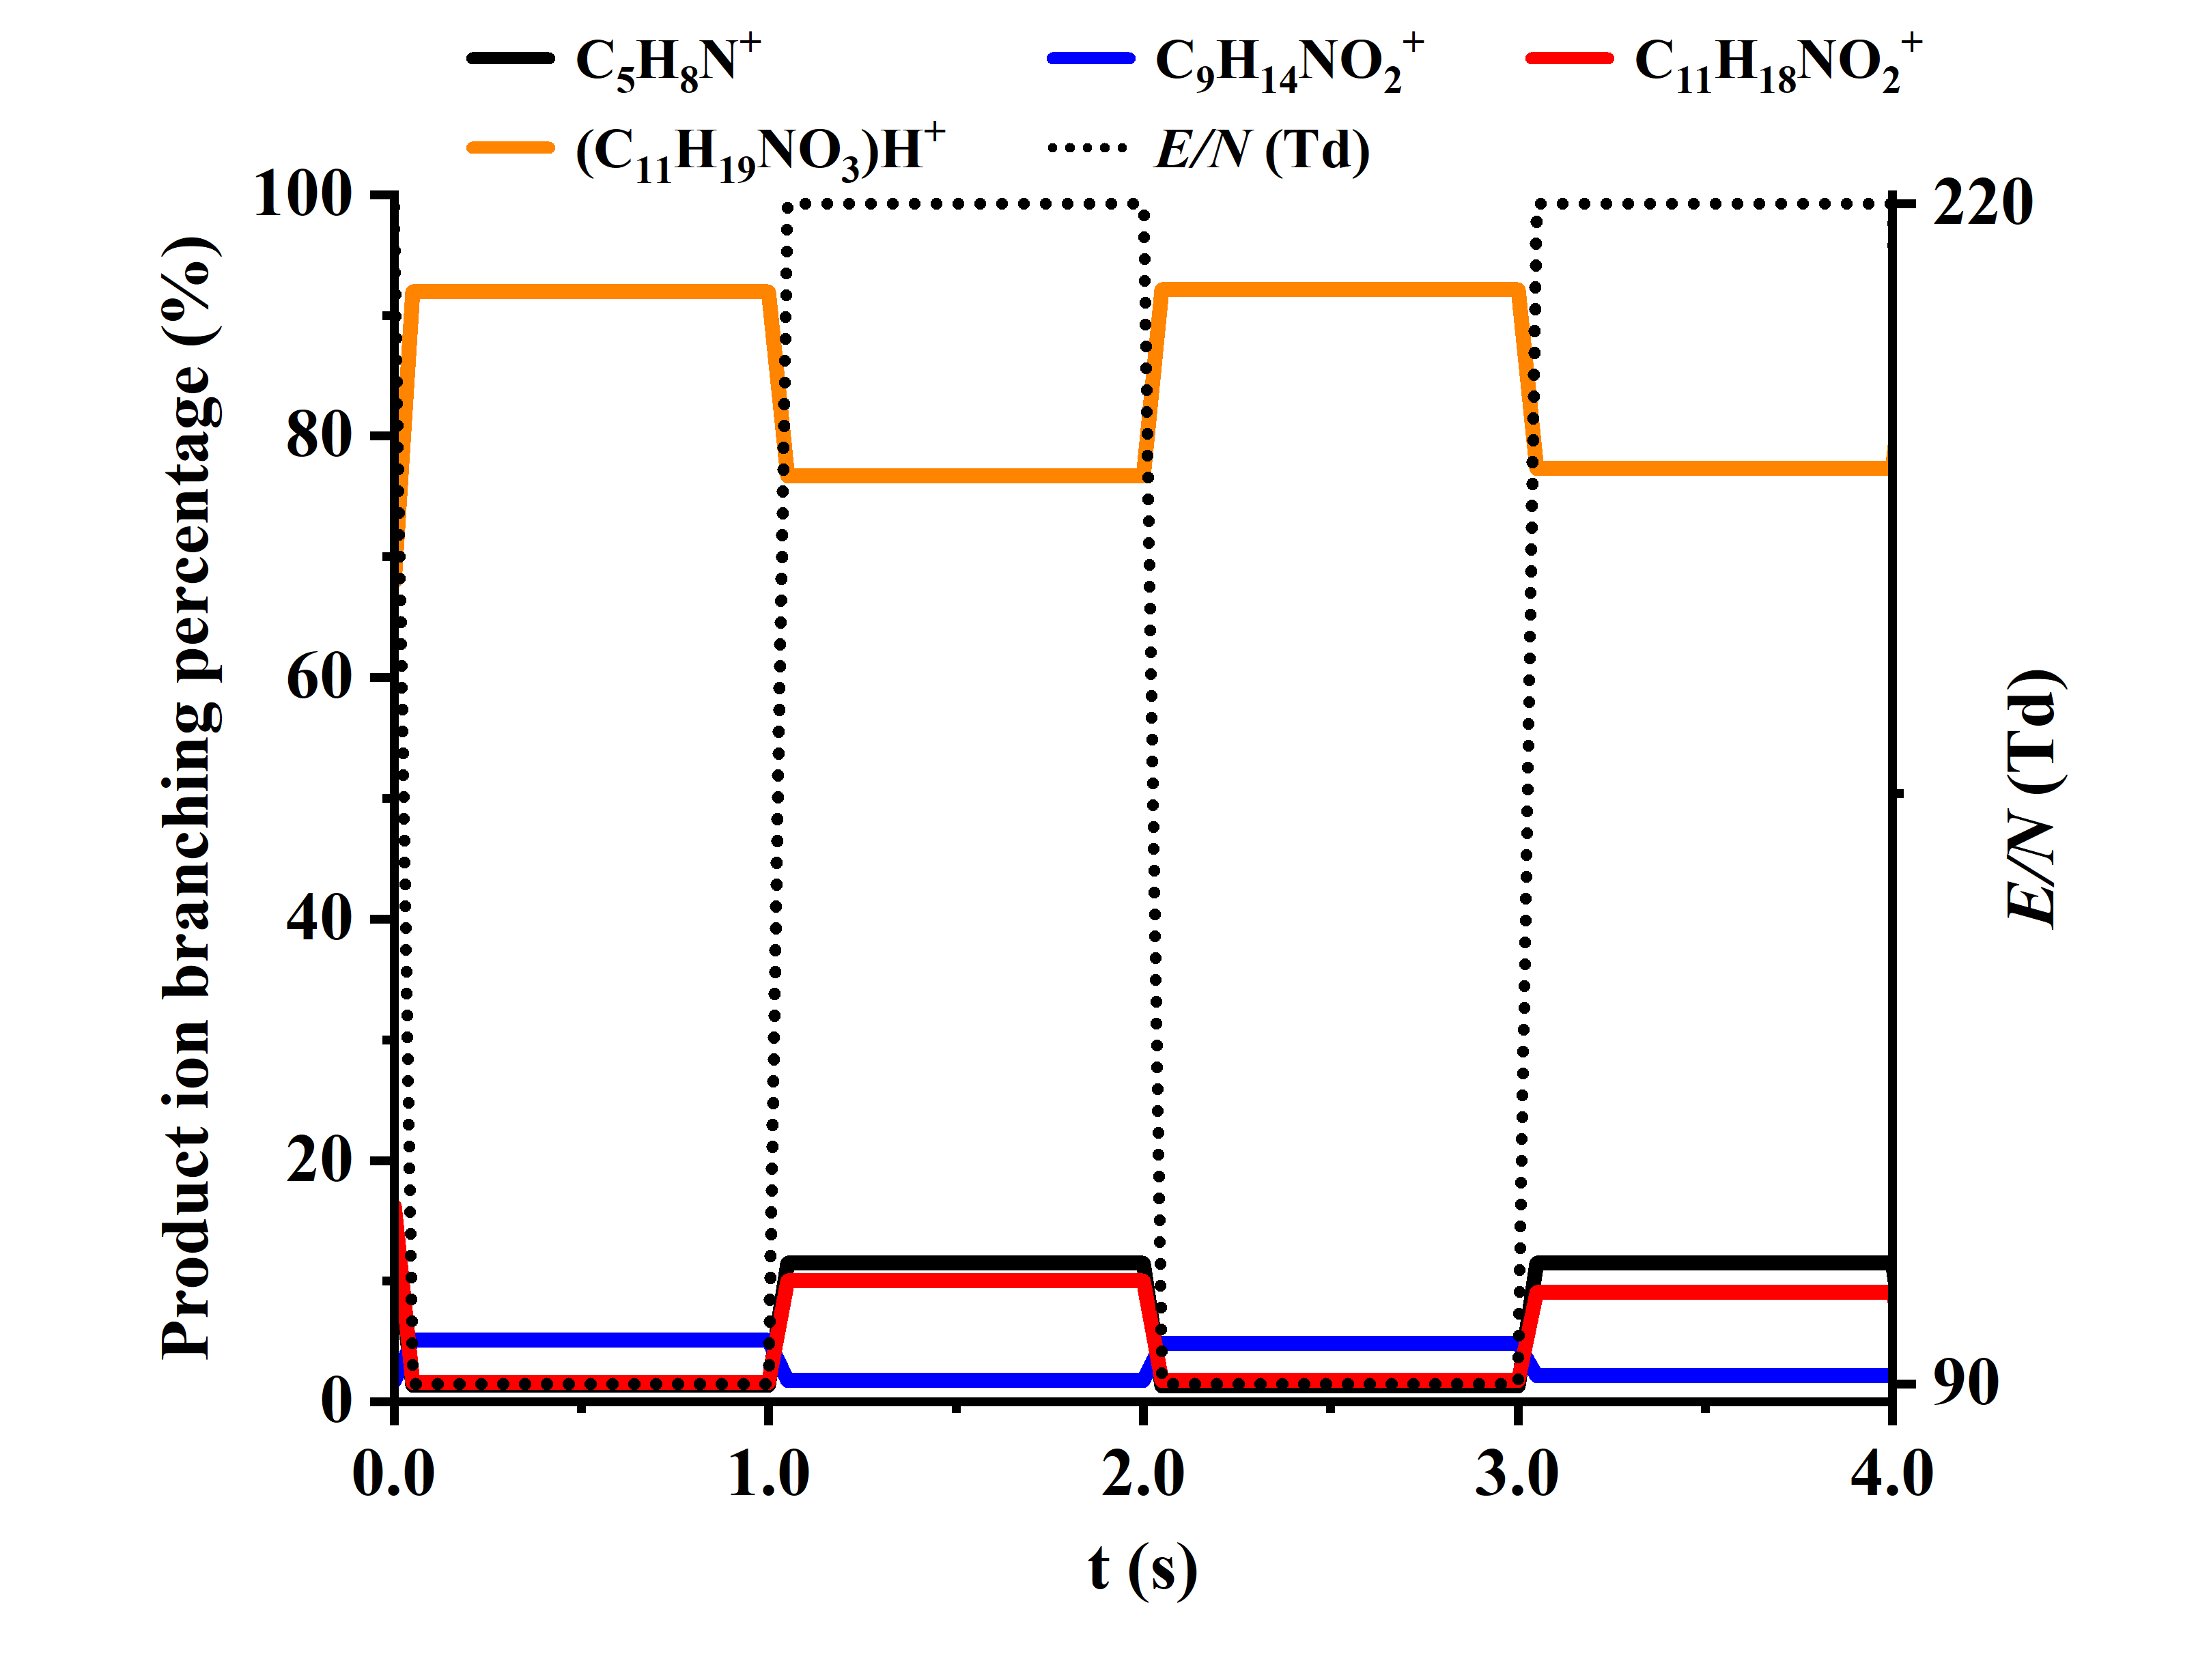
\includegraphics[width=0.80\linewidth]{pics/other_drugs/EtEcg-fs-90-220.png}
\caption{Ethyl ecgonine reduced electric field fast switching plot.}
\label{fig:DR_EtEcg_fs}
\end{figure}


\begin{figure}[htb]
\centering
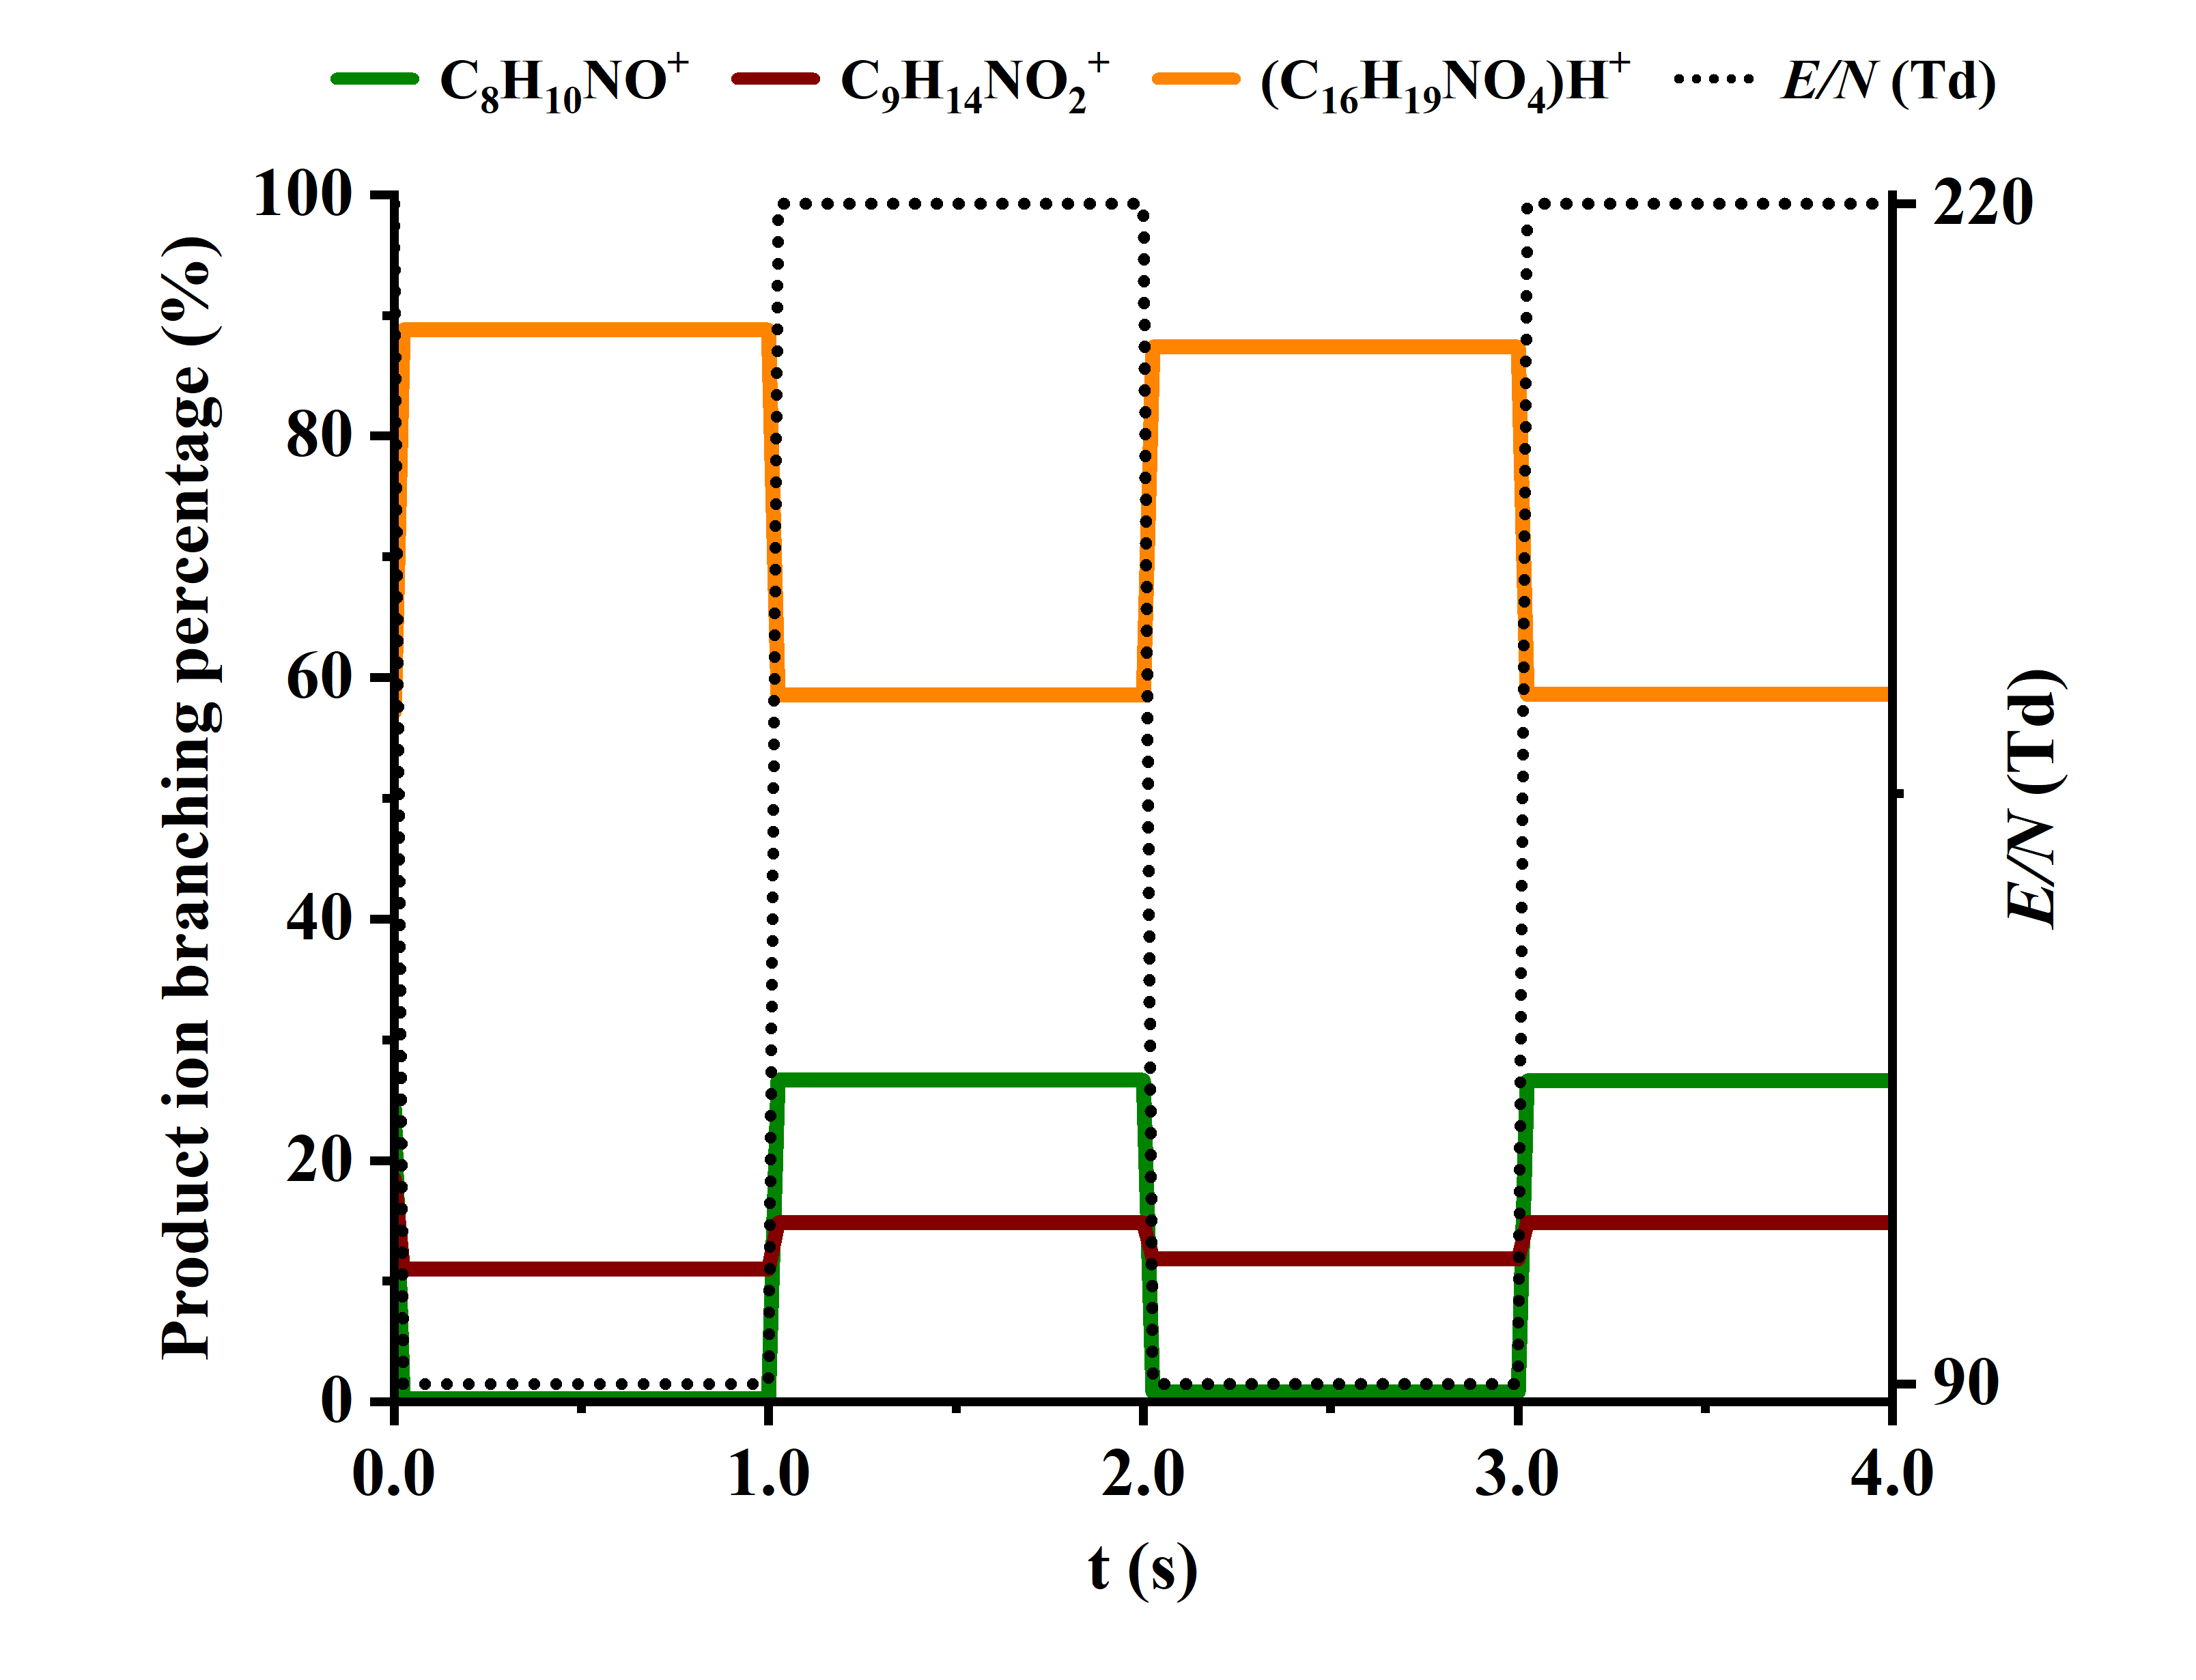
\includegraphics[width=0.80\linewidth]{pics/other_drugs/norcocaine-fs-90-220.png}
\caption{Norcocaine reduced electric field fast switching plot.}
\label{fig:DR_norcocaine_fs}
\end{figure}


\begin{figure}[htb]
\centering
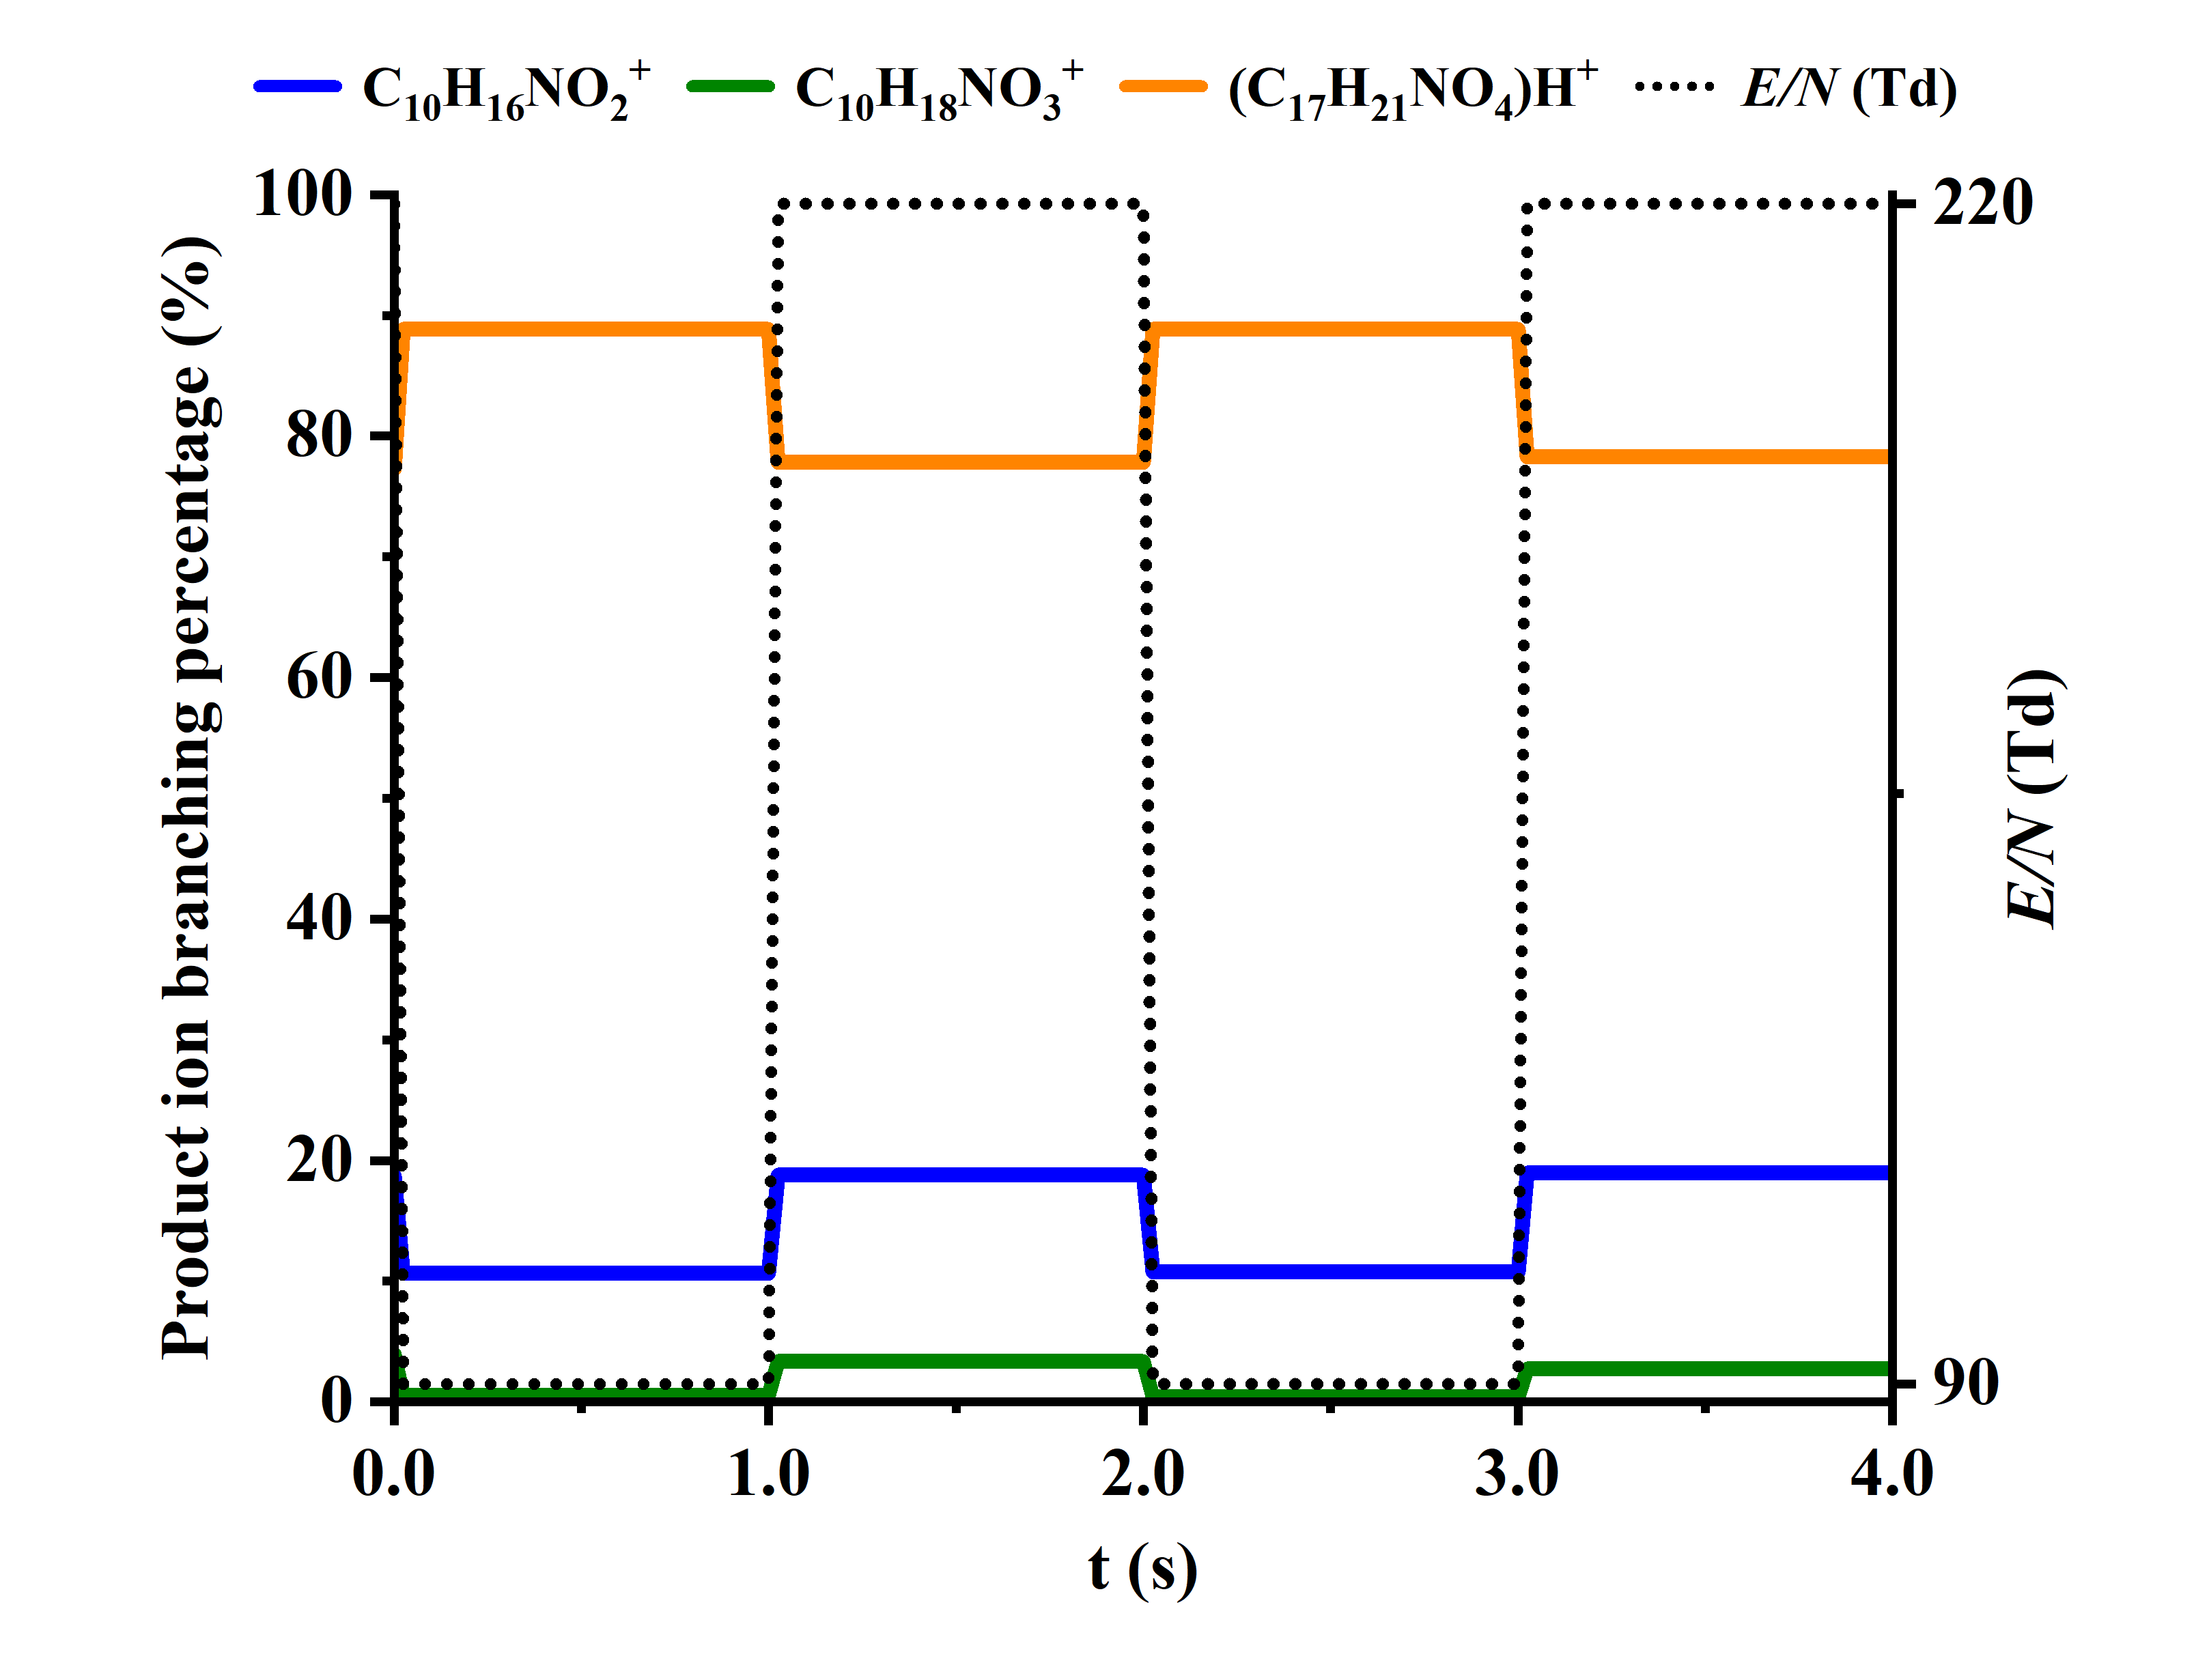
\includegraphics[width=0.80\linewidth]{pics/other_drugs/ohcocaine-fs-90-220.png}
\caption{o-Hydroxycocaine reduced electric field fast switching plot.}
\label{fig:DR_ohcocaine_fs}
\end{figure}



\begin{figure}[htb]
\centering
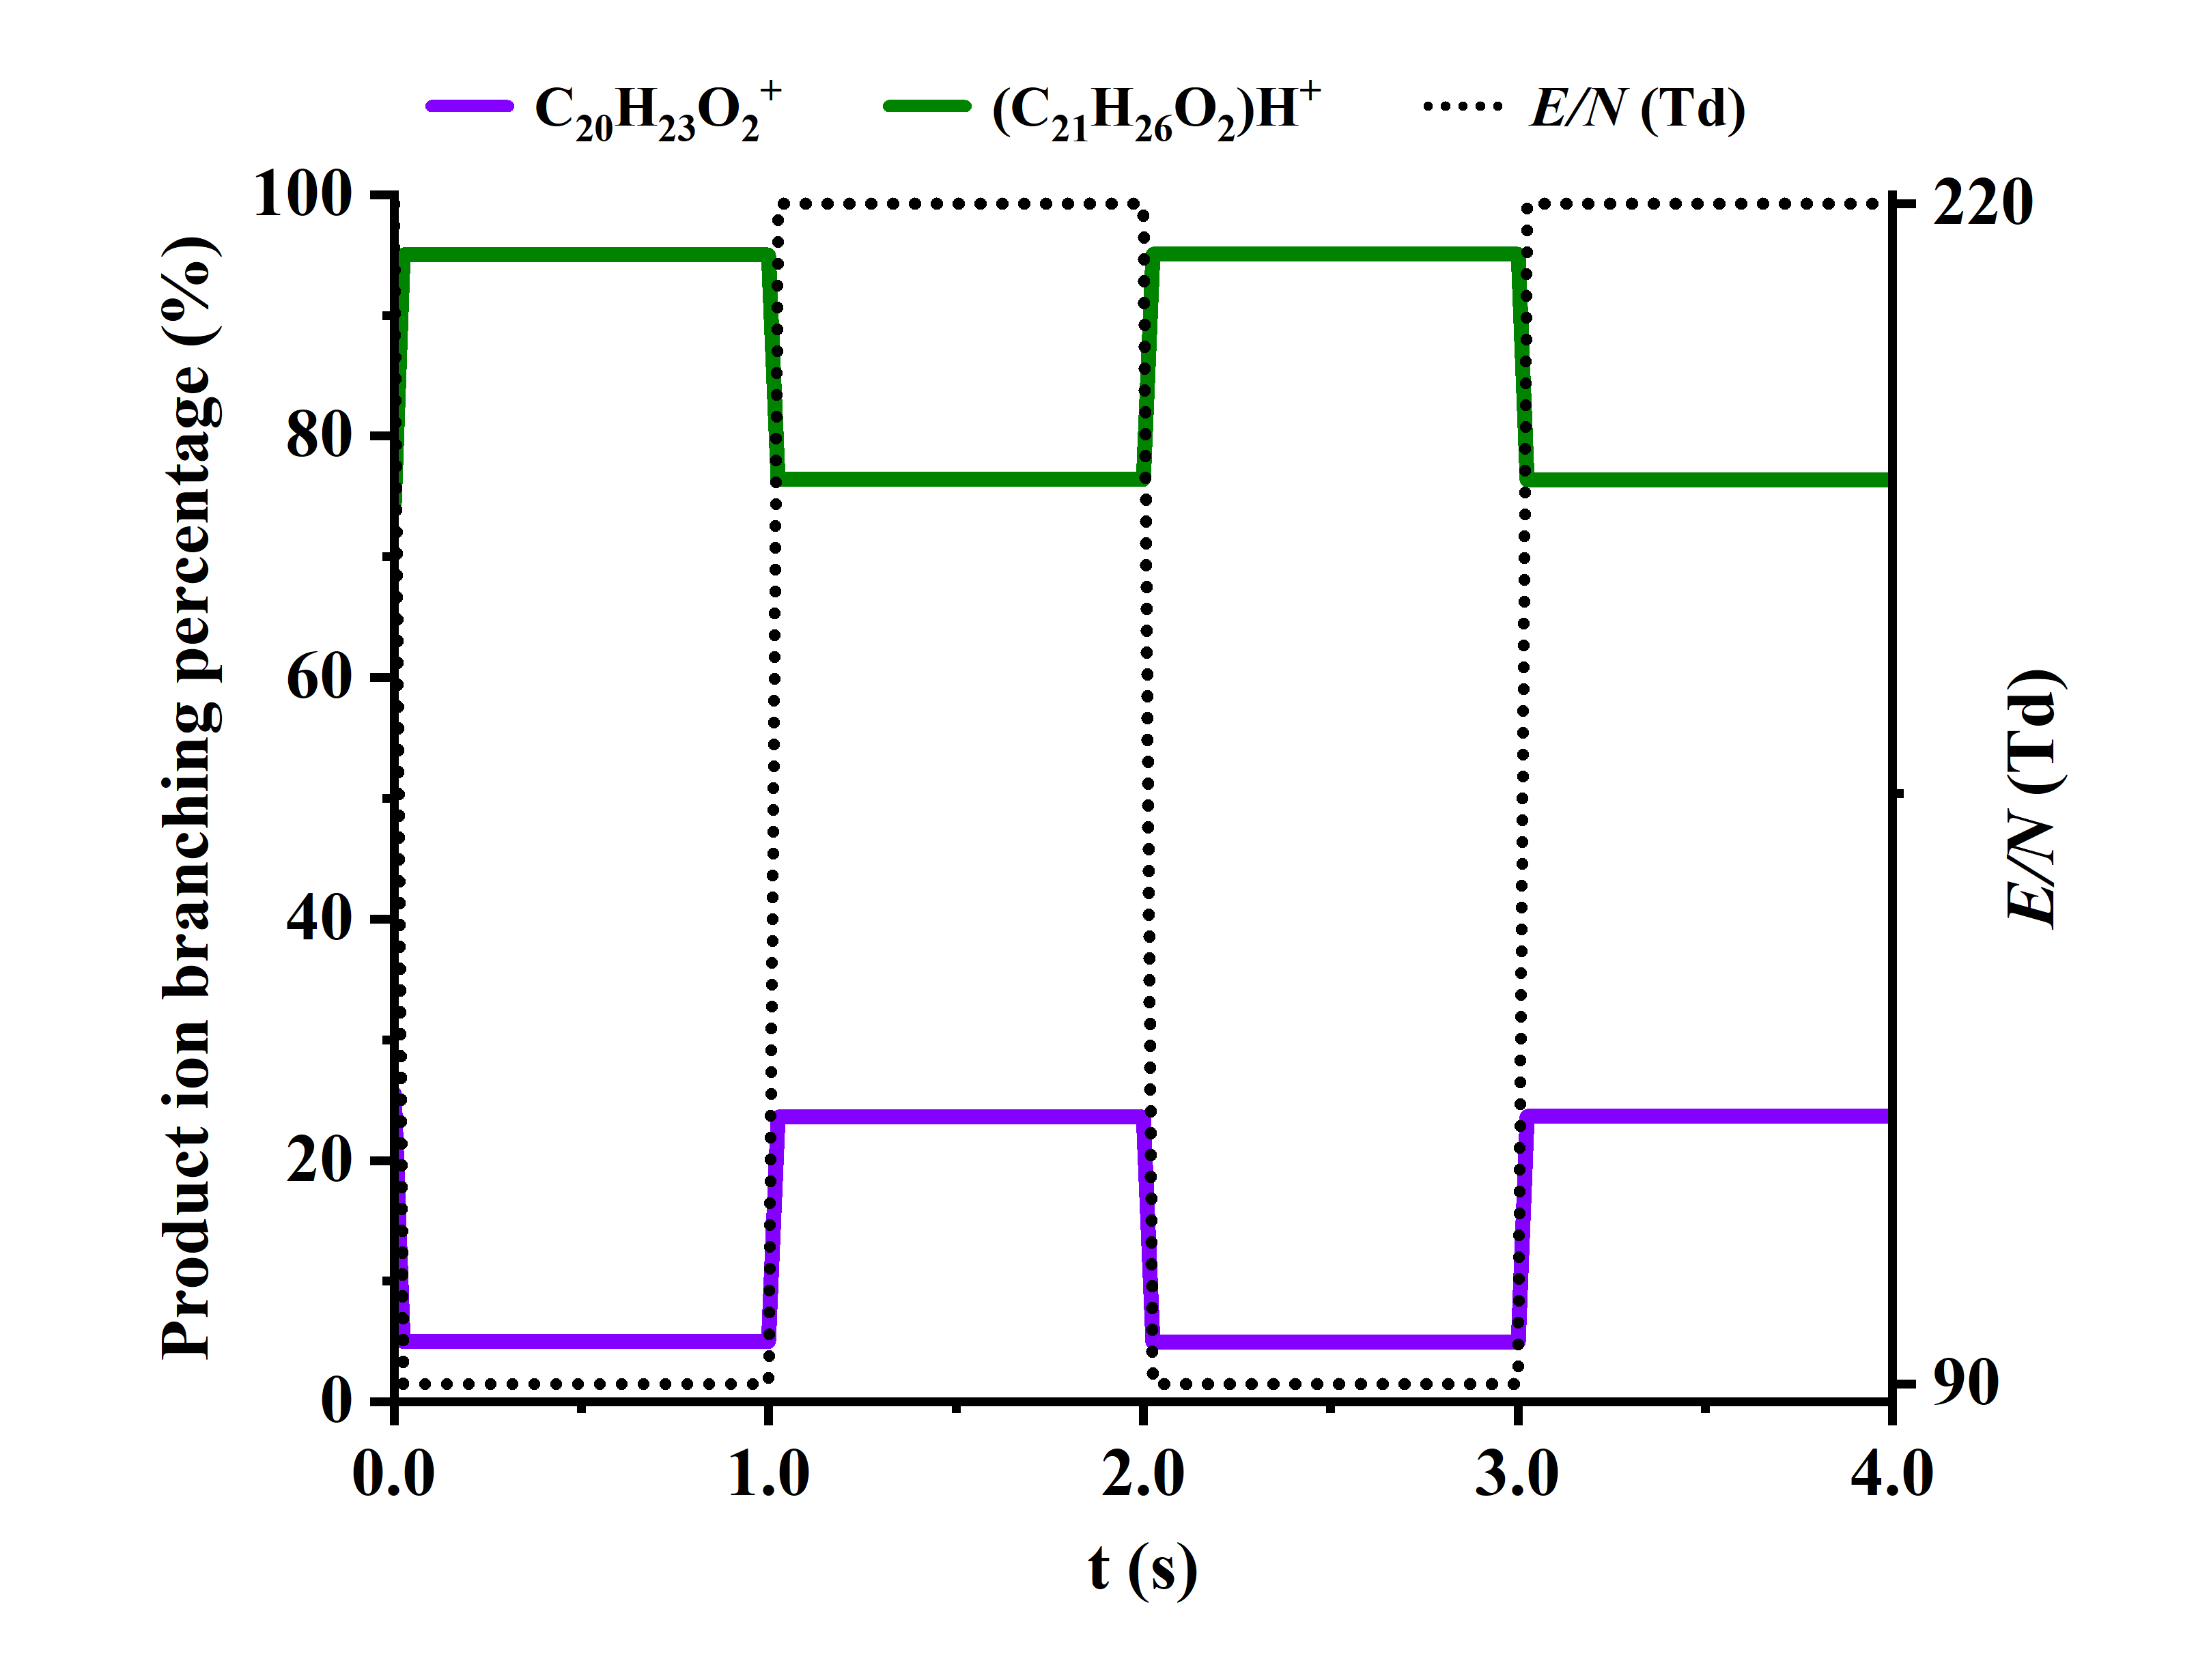
\includegraphics[width=0.80\linewidth]{pics/other_drugs/CBN-fs-90-220.png}
\caption{CBN reduced electric field fast switching plot.}
\label{fig:DR_CBN_fs}
\end{figure}



\begin{figure}[htb]
\centering
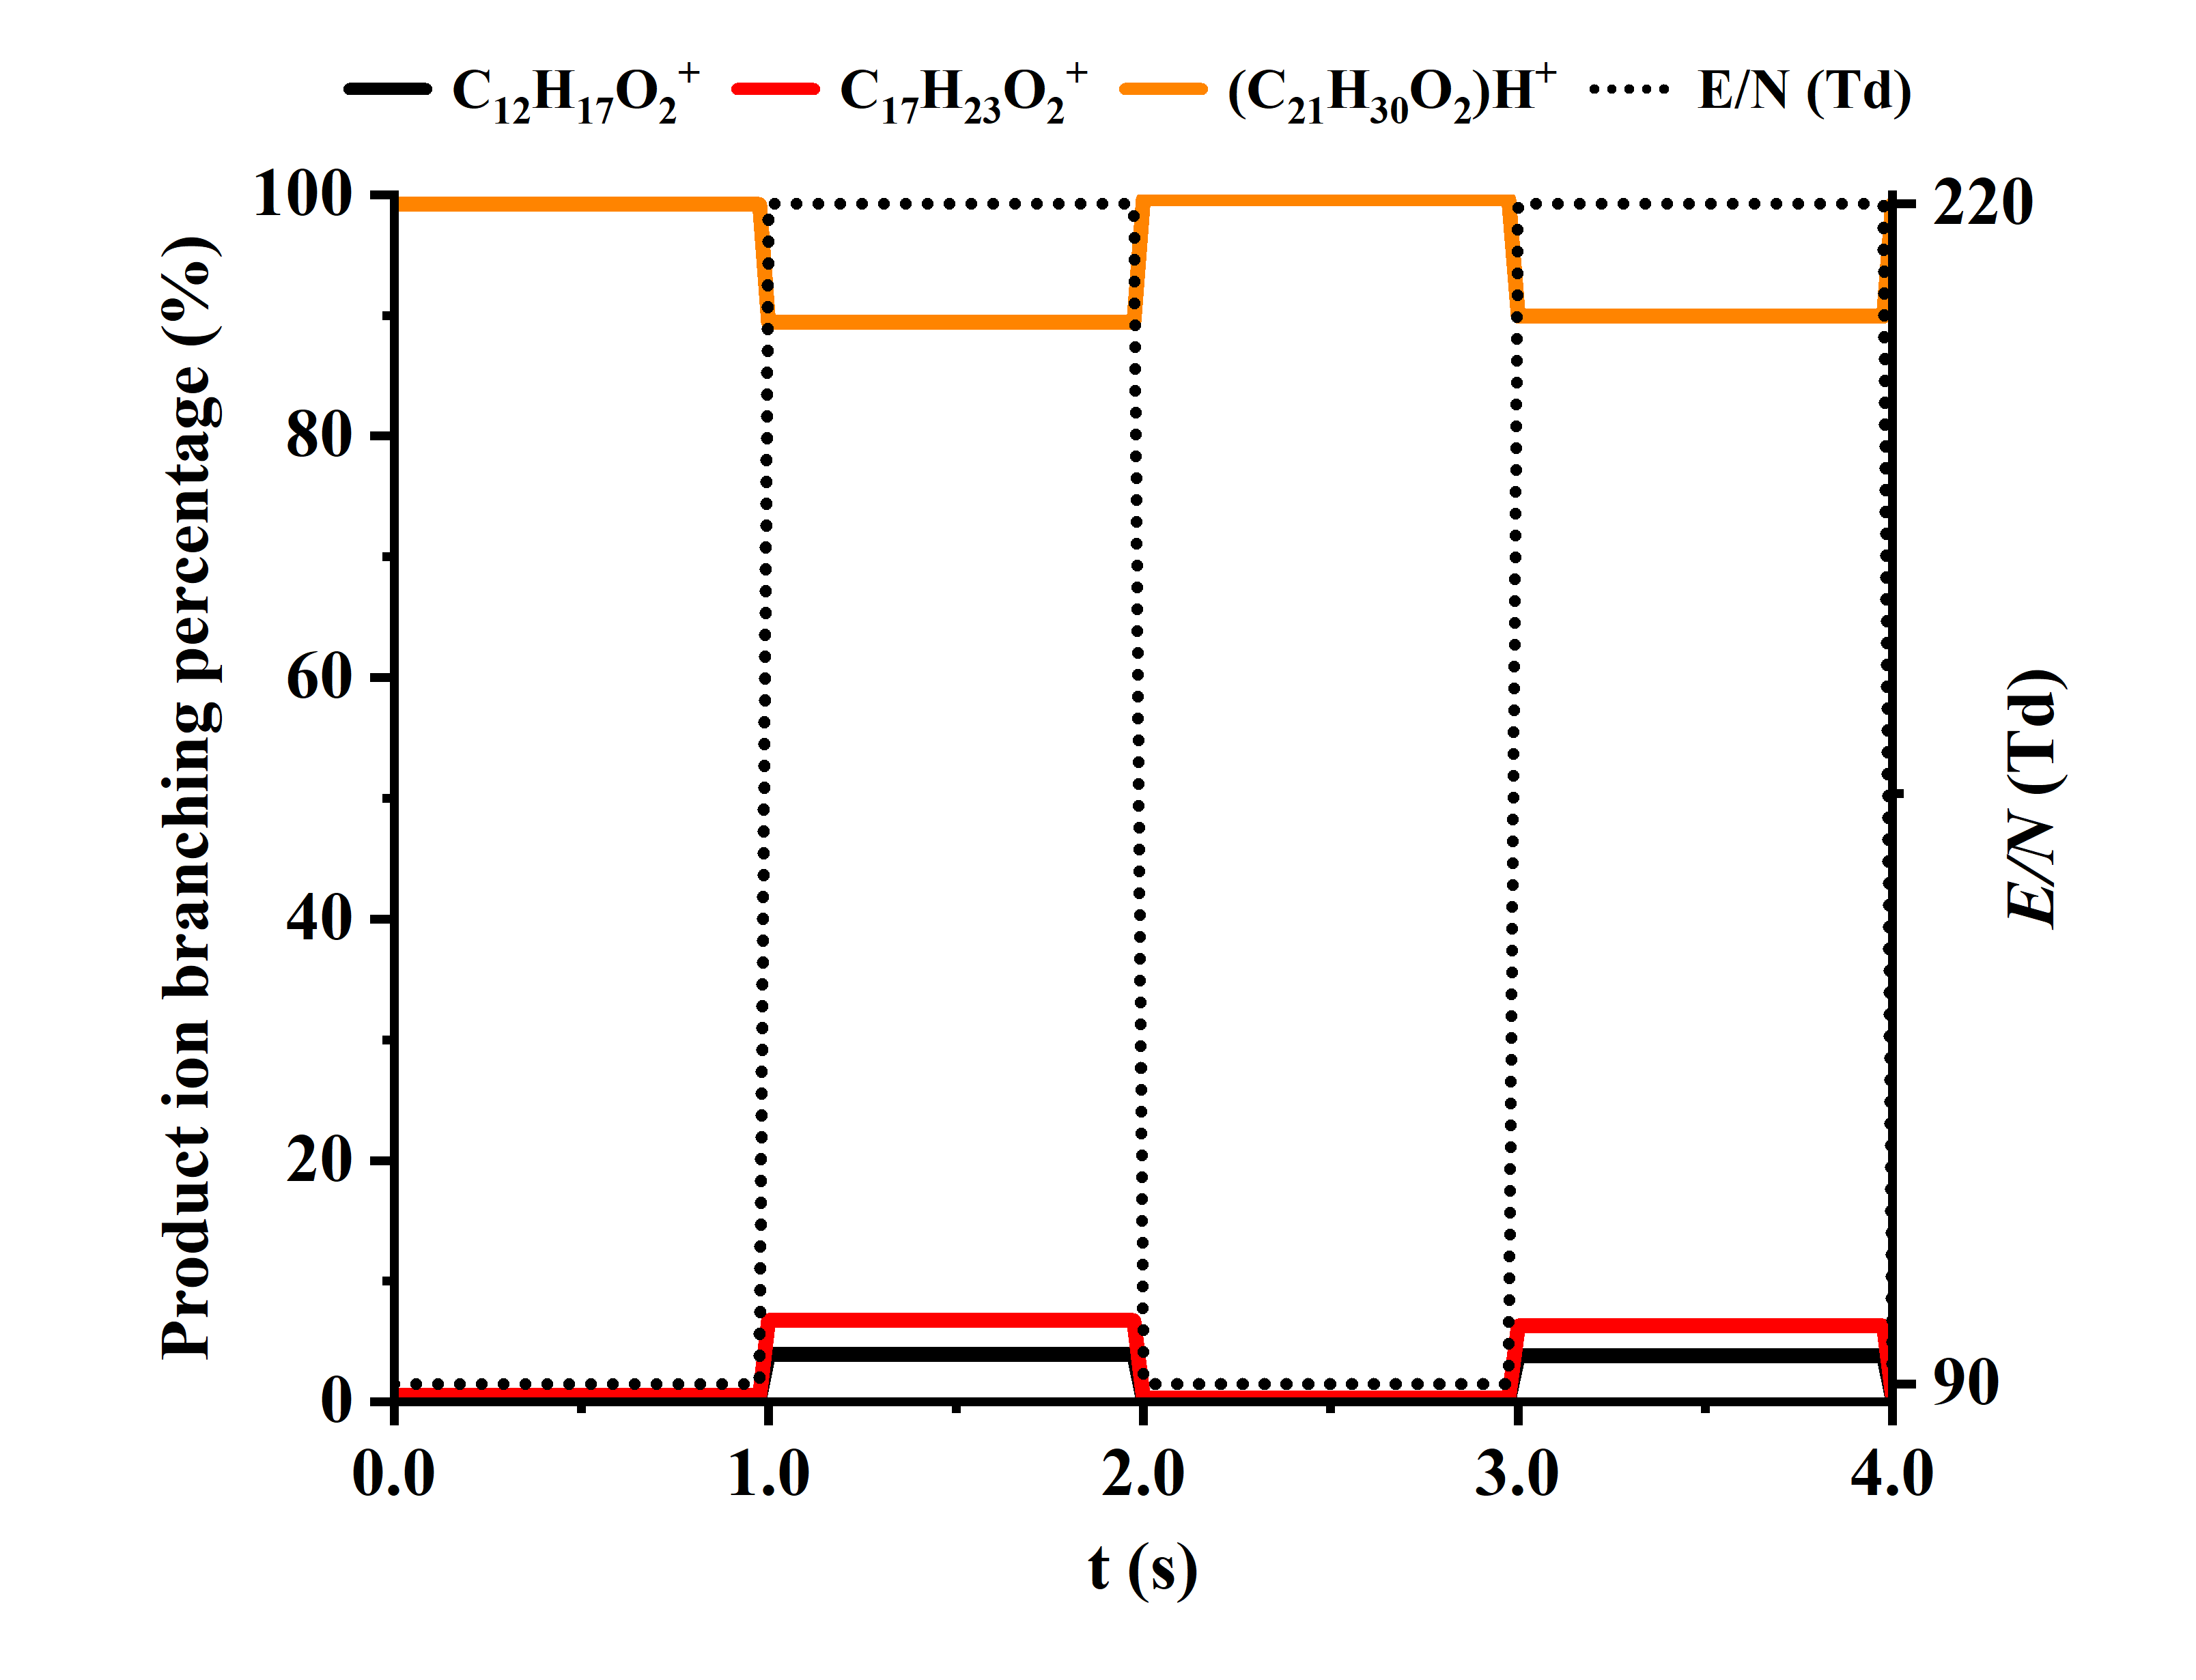
\includegraphics[width=0.80\linewidth]{pics/other_drugs/THC-fs-90-220.png}
\caption{$\Delta$-9-THC reduced electric field fast switching plot.}
\label{fig:DR_THC_fs}
\end{figure}



\begin{figure}[htb]
\centering
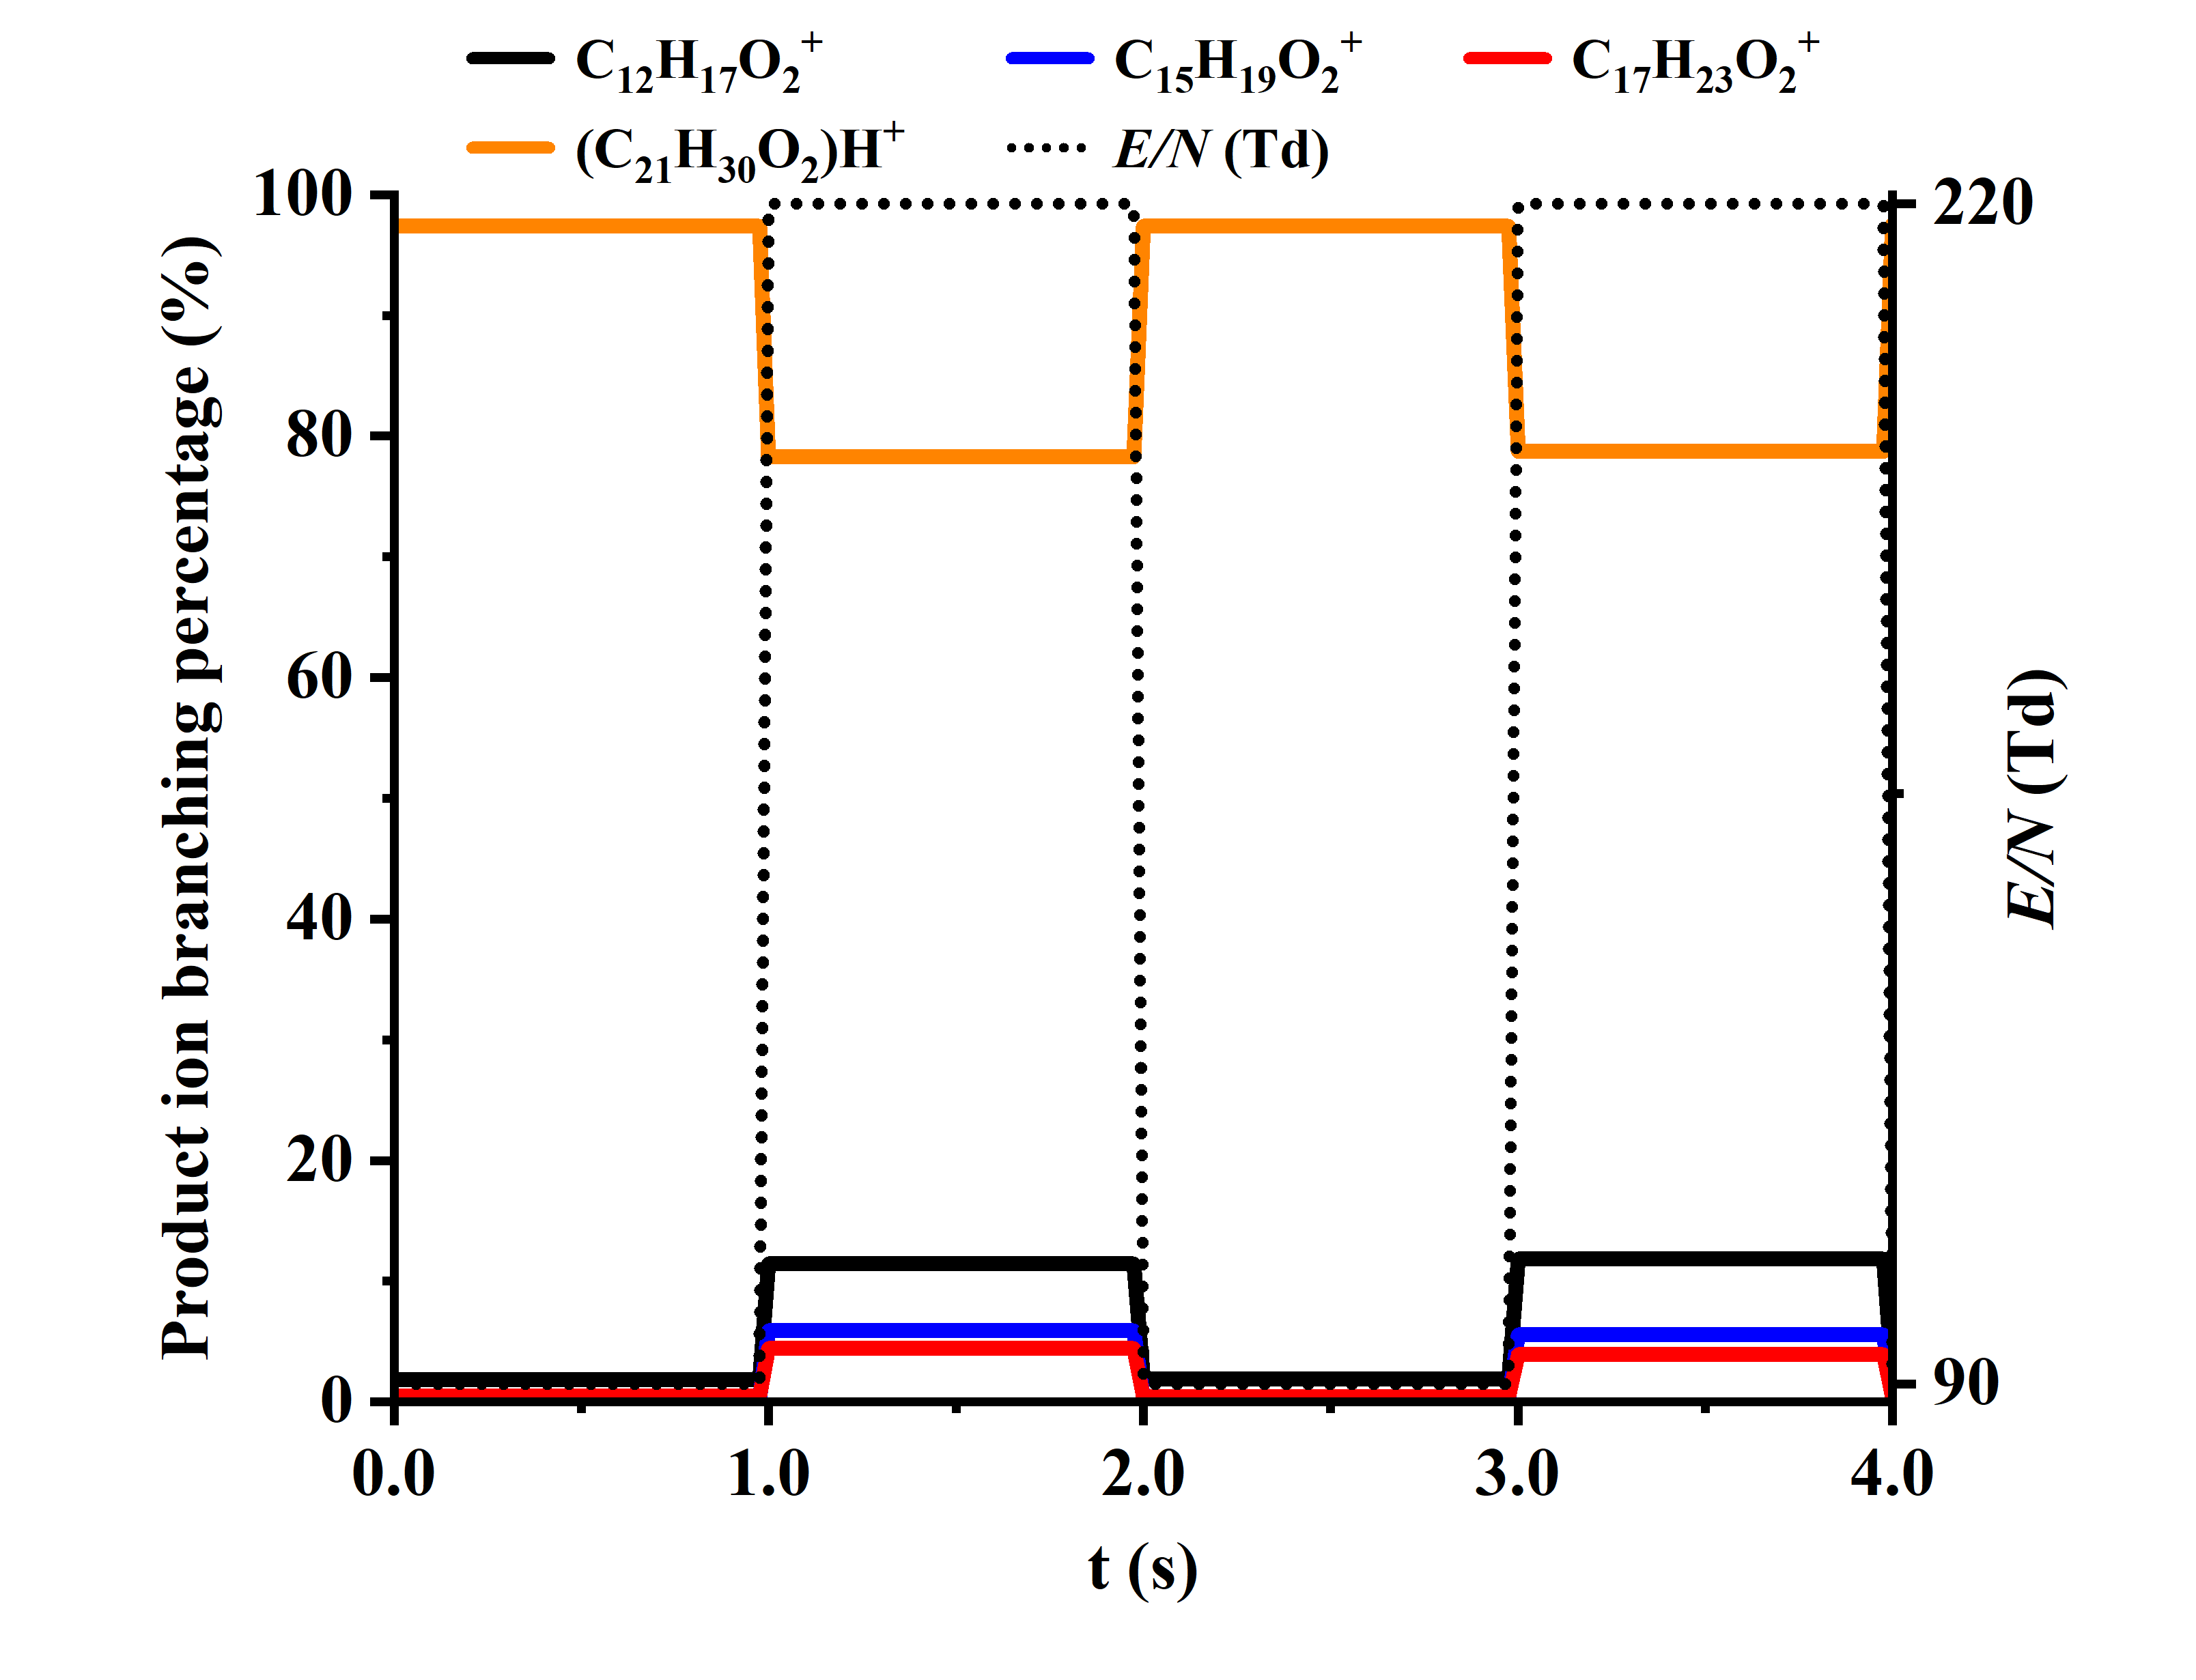
\includegraphics[width=0.80\linewidth]{pics/other_drugs/CBD-fs-90-220.png}
\caption{CBD reduced electric field fast switching plot.}
\label{fig:DR_CBD_fs}
\end{figure}














